\documentclass[12pt]{amsart}

%Below are some necessary packages for your course.
\usepackage{amsfonts,latexsym,amsthm,amssymb,amsmath,amscd,euscript}
\usepackage{framed}
\usepackage{fullpage}
\usepackage{hyperref}
    \hypersetup{colorlinks=true,citecolor=blue,urlcolor =black,linkbordercolor={1 0 0}}
\usepackage{mathtools}
\usepackage[table]{xcolor}
% For drawing Venn diagrams with patterns for shading
\usepackage{tikz}
\usetikzlibrary{patterns}
\definecolor{zesty orange}{rgb}{0.9608, 0.4745, 0.2274}
\definecolor{zesty blue}{rgb}{0.5216, 0.7529, 0.9765}
\definecolor{zesty purple}{rgb}{0.6627, 0.3529, 0.6314}

\newenvironment{statement}[1]{\smallskip\noindent\color[rgb]{.6627, .3529, .6314} {\bf #1.}}{}
\allowdisplaybreaks[1]

%Below are the theorem, definition, example, lemma, etc. body types.

\newtheorem{theorem}{Theorem}
\newtheorem*{proposition}{Proposition}
\newtheorem{lemma}[theorem]{Lemma}
\newtheorem{corollary}[theorem]{Corollary}
\newtheorem{conjecture}[theorem]{Conjecture}
\newtheorem{postulate}[theorem]{Postulate}
\theoremstyle{definition}
\newtheorem{defn}[theorem]{Definition}
\newtheorem{example}[theorem]{Example}

\theoremstyle{remark}
\newtheorem*{remark}{Remark}
\newtheorem*{notation}{Notation}
\newtheorem*{note}{Note}

% You can define new commands to make your life easier.
\newcommand{\BR}{\mathbb R}
\newcommand{\BC}{\mathbb C}
\newcommand{\BF}{\mathbb F}
\newcommand{\BQ}{\mathbb Q}
\newcommand{\BZ}{\mathbb Z}
\newcommand{\BN}{\mathbb N}

% We can even define a new command for \newcommand!
\newcommand{\nc}{\newcommand}

% If you want a new function, use operatorname to define that function (don't use \text)
\nc{\on}{\operatorname}
\nc{\Spec}{\on{Spec}}

\title{\emph{How to Prove It}: Chapter 1} % IMPORTANT: Change the problemset number as needed.
\date{\today}

\begin{document}

\maketitle

\vspace*{-0.25in}
\centerline{Kyle Stratton}

\begin{framed}
These are the exercises for Chapter 1 from the third edition of \emph{How to Prove It} by Daniel J. Velleman.
They are numbered (Chapter).(Section).(Exercise).
\end{framed}

\begin{statement}{1.1.1}
Analyze the logical forms of the following statements:
\begin{enumerate}
	\item We'll have either a reading assignment or homework problems, but we won't have both homework problems and a test.
	\item You won't go skiing, or you will and there won't be any snow.
	\item $\sqrt{7} \nleq 2$.
\end{enumerate}
\end{statement}

\begin{proof}
\hfill
\begin{enumerate}
	\item Let $R$ be the statement ``We'll have a reading assignment," $H$ the statement ``We'll have homework problems,'' and $T$ the statement ``We'll have a test.''
	This statement has the logical form $(R \vee H) \wedge \neg (H \wedge T)$.
	
	\item Let $P$ be the statement ``You will go skiing,'' and $Q$ the statement ``There will be snow.''
	This statement has the logical form $\neg P \vee (P \wedge \neg Q)$.
	
	\item We'll use some notation that shows up in Chapter 1.3.
	Let $P(x, y)$ be the statement ``$x < y$'' and $Q(x, y)$ the statement ``$x = y$.''
	This statement has the logical form $P(\sqrt{7}, 2) \wedge \neg Q(\sqrt{7}, 2)$.
\end{enumerate}
\end{proof}


\begin{statement}{1.1.2}
Analyze the logical forms of the following statements:
\begin{enumerate}
	\item Either John and Bill are both telling the truth, or neither of them is.
	\item I'll have either fish or chicken, but I won't have both fish and mashed potatoes.
	\item 3 is a common divisor of 6, 9, and 15.
\end{enumerate}
\end{statement}

\begin{proof}
\hfill
\begin{enumerate}
	\item Let $J$ be the statement ``John is telling the truth,'' and $B$ the statement ``Bill is telling the truth.''
	This statement has the logical form $(J \wedge B) \vee (\neg J \wedge \neg B)$.
	
	\item Let $F$ be the statement ``I'll have fish,'' $C$ the statement ``I'll have chicken,'' and $M$ the statement ``I'll have mashed potatoes.''
	This statement has the logical form $(F \vee C) \wedge \neg (F \wedge M)$.
	
	\item Let $P(x)$ be the statement ``3 divides $x$.''
	This statement has the logical form $P(6) \wedge P(9) \wedge P(15)$.
\end{enumerate}
\end{proof}


\begin{statement}{1.1.3}
Analyze the logical forms of the following statements:
\begin{enumerate}
	\item Alice and Bob are not both in the room.
	\item Alice and Bob are both not in the room.
	\item Either Alice or Bob is not in the room.
	\item Neither Alice nor Bob is in the room.
\end{enumerate}
\end{statement}

\begin{proof}
Let $A$ be the statement ``Alice is in the room,'' and $B$ the statement ``Bob is in the room.''
Then the above statements have the following logical forms.
\begin{enumerate}
	\item $\neg (A \wedge B)$
	\item $\neg A \wedge \neg B$
	\item $\neg A \vee \neg B$
	\item $\neg (A \vee B)$
\end{enumerate}
\end{proof}


\begin{statement}{1.1.4}
Analyze the logical forms of the following statements:
\begin{enumerate}
	\item Either both Ralph and Ed are tall, or both of them are handsome.
	\item Both Ralph and Ed are either tall or handsome.
	\item Both Ralph and Ed are neither tall nor handsome.
	\item Neither Ralph nor Ed is both tall and handsome.
\end{enumerate}
\end{statement}

\begin{proof}
Let $R_T$ be the statement ``Ralph is tall,'' $R_H$ the statement ``Ralph is handsome,'' $E_T$ the statement ``Ed is tall,'' and $E_H$ the statement ``Ed is handsome.
Then the above statements have the following logical forms.
\begin{enumerate}
	\item $(R_T \wedge E_T) \vee (R_H \wedge E_H)$
	\item $(R_T \vee R_H) \wedge (E_T \vee E_H)$
	\item $(\neg R_T \wedge \neg R_H) \wedge (\neg E_T \wedge \neg E_H)$
	\item $\neg (R_T \wedge R_H) \wedge \neg (E_T \wedge E_H)$
\end{enumerate}
\end{proof}


\begin{statement}{1.1.5}
Which of the following expressions are well-formed formulas?
\begin{enumerate}
	\item $\neg ( \neg P \vee \neg \neg R )$.
	\item $\neg ( P, Q, \wedge R )$.
	\item $P \wedge \neg P$.
	\item $(P \wedge Q)(P \vee R)$.
\end{enumerate}
\end{statement}

\begin{proof}
Only formulas (1) and (3) are well-formed.
\end{proof}


\begin{statement}{1.1.6}
Let $P$ stand for the statement ``I will buy the pants'' and $S$ for the statement ``I will buy the shirt.''
What English sentences are represented by the following formulas?
\begin{enumerate}
	\item $\neg (P \wedge \neg S)$.
	\item $\neg P \wedge \neg S$.
	\item $\neg P \vee \neg S$.
\end{enumerate}
\end{statement}

\begin{proof}
\hfill
\begin{enumerate}
	\item I will not buy the pants without buying the shirt.
	\item I will not buy the pants and I will not buy the shirt.
	\item Either I won't buy the pants or I won't buy the shirt.
\end{enumerate}
\end{proof}


\begin{statement}{1.1.7}
Let $S$ stand for the statement ``Steve is happy'' and $G$ for ``George is happy.''
What English sentences are represented by the following formulas?
\begin{enumerate}
	\item $(S \vee G) \wedge (\neg S \vee \neg G)$.
	\item $[S \vee (G \wedge \neg S)] \vee \neg G$.
	\item $S \vee [G \wedge (\neg S \vee \neg G)]$.
\end{enumerate}
\end{statement}

\begin{proof}
\hfill
\begin{enumerate}
	\item Either Steve or George is happy, but they are not both happy.
	\item Steve is happy, or Steve is unhappy while George is happy, or George is unhappy.
	\item Steve is happy, or George is happy and either Steve or George is unhappy.
	\emph{Note that this sentence can be simplified to ``Steve or George is happy.''}
\end{enumerate}
\end{proof}


\begin{statement}{1.1.8}
Let $T$ stand for the statement ``Taxes will go up'' and $D$ for ``The deficit will go up.''
What English sentences are represented by the following formulas?
\begin{enumerate}
	\item $T \vee D$.
	\item $\neg (T \wedge D) \wedge \neg (\neg T \wedge \neg D)$.
	\item $(T \wedge \neg D) \vee (D \wedge \neg T)$.
\end{enumerate}
\end{statement}

\begin{proof}
\hfill
\begin{enumerate}
	\item Taxes will go up or the deficit deficit will go up.
	\item Taxes and the deficit won't both go up, and they also won't both not go up.
	\item Either taxes will go up and the deficit won't, or the deficit will go up and taxes won't.
\end{enumerate}
\end{proof}


\begin{statement}{1.1.9}
Identify the premises and conclusions of the following deductive arguments and analyze their logical forms.
Do you think the reasoning is valid?
(Although you will have only your intuition to guide you in answering this last question, in the next section we will develop some techniques for determining the validity of arguments.)
\begin{enumerate}
	\item Jane and Pete won't both win the math prize.
	Pete will win either the math prize or the chemistry prize.
	Jane will win the math prize.
	Therefore, Pete will win the chemistry prize.
	
	\item The main course will be either beef or fish.
	The vegetable will be either peas or corn.
	We will not have both fish as a main course and corn as a vegetable.
	Therefore, we will not have both beef as a main course and peas as a vegetable.
	
	\item Either John or Bill is telling the truth.
	Either Sam or Bill is lying.
	Therefore either John is telling the truth or Sam is lying.
	
	\item Either sales will go up and the boss will be happy, or expenses will go up and the boss won't be happy.
	Therefore, sales and expenses will not both go up.
\end{enumerate}
\end{statement}

\begin{proof}
\hfill
\begin{enumerate}
	\item Let $J_M$ be the statement ``Jane will win the math prize,'' $P_M$ the statement ``Pete will win the math prize,'' and $P_C$ the statement ``Pete will win the chemistry prize.''
	Then the deductive argument takes the following form.
	\begin{equation*}
		\begin{array}{l}
			\neg (J_M \wedge P_M) \\
			P_M \vee P_C \\
			J_M \\
			\hline
			\therefore P_C
		\end{array}
	\end{equation*}
	This argument appears to be valid.
	
	\item Let $B$ be the statement ``The main course will be beef,'' $F$ the statement ``The main course will be fish,'' $P$ the statement ``The vegetable will be peas,'' and $C$ the statement ``The vegetable will be corn.''
	Then the deductive argument takes the following form.
	\begin{equation*}
		\begin{array}{l}
			B \vee F \\
			P \vee C \\
			\neg (F \wedge C) \\
			\hline
			\therefore \neg (B \wedge P)
		\end{array}
	\end{equation*}
	This argument does not appear to be valid because not having fish and corn together says nothing about the pairing of beef with peas.
	
	\item Let $J$ be the statement ``John is telling the truth,'' $B$ the statement ``Bill is telling the truth,'' and $S$ the statement ``Sam is telling the truth.''
	Then the deductive argument takes the following form.
	\begin{equation*}
		\begin{array}{l}
			J \vee B \\
			\neg S \vee \neg B \\
			\hline
			\therefore J \vee \neg S
		\end{array}
	\end{equation*}
	This argument appears to be valid because if John is lying and Sam is telling the truth, then one of the premises must be false, as Bill cannot be simultaneously telling the truth and lying.
	
	\item Let $S$ be the statement ``Sales will go up,'' $E$ the statement ``Expenses will go up,'' and $B$ the statement ``The boss will be happy.''
	Then the deductive argument takes the following form.
	\begin{equation*}
		\begin{array}{l}
			(S \wedge B) \vee (E \wedge \neg B) \\
			\hline
			\therefore \neg (S \wedge E)
		\end{array}
	\end{equation*}
	This argument does not appear to be valid because the boss's state of happiness or unhappiness doesn't necessarily influence the increase of sales or expenses.
\end{enumerate}
\end{proof}


\begin{statement}{1.2.1}
Make truth tables for the following formulas:
\begin{enumerate}
	\item $\neg P \vee Q$.
	\item $(S \vee G) \wedge (\neg S \vee \neg G)$.
\end{enumerate}
\end{statement}

\begin{proof}
\hfill
\begin{enumerate}
	\item 
	\begin{equation*}
		\begin{array}{| c c | c |}
			P & Q & \neg P \vee Q \\
			\hline
			T & T & F \vee T = T \\
			T & F & F \vee F = F \\
			F & T & T \vee T = T \\
			F & F & T \vee F = T
		\end{array}
	\end{equation*}
	
	\item 
	\begin{equation*}
		\begin{array}{| c c | c |}
			S & G & (S \vee G) \wedge (\neg S \vee \neg G) \\
			\hline
			T & T & (T \vee T) \wedge (F \vee F) = T \wedge F = F \\
			T & F & (T \vee F) \wedge (F \vee T) = T \wedge T = T \\
			F & T & (F \vee T) \wedge (T \vee F) = T \wedge T = T \\
			F & F & (F \vee F) \wedge (T \vee T) = F \wedge T = F
		\end{array}
	\end{equation*}
\end{enumerate}
\end{proof}


\begin{statement}{1.2.2}
Make truth tables for the following formulas:
\begin{enumerate}
	\item $\neg [P \wedge (Q \vee \neg P)]$.
	\item $(P \vee Q) \wedge (\neg P \vee R)$.
\end{enumerate}
\end{statement}

\begin{proof}
\hfill
\begin{enumerate}
	\item 
	\begin{equation*}
		\begin{array}{| c c | c |}
			P & Q & \neg [P \wedge (Q \vee \neg P)] \\
			\hline
			T & T & \neg [T \wedge (T \vee F)] = F \\
			T & F & \neg [T \wedge (F \vee T)] = F \\
			F & T & \neg [F \wedge (T \vee F)] = T \\
			F & F & \neg [F \wedge (F \vee T)] = T
		\end{array}
	\end{equation*}
	
	\item 
	\begin{equation*}
		\begin{array}{| c c c | c |}
			P & Q & R & (P \vee Q) \wedge (\neg P \vee R) \\
			\hline
			T & T & T & (T \vee T) \wedge (F \vee T) = T \\
			T & T & F & (T \vee T) \wedge (F \vee F) = F \\
			T & F & T & (T \vee F) \wedge (F \vee T) = T \\
			T & F & F & (T \vee F) \wedge (F \vee F) = F \\
			F & T & T & (F \vee T) \wedge (T \vee T) = T \\
			F & T & F & (F \vee T) \wedge (T \vee F) = T \\
			F & F & T & (F \vee F) \wedge (T \vee T) = F \\
			F & F & F & (F \vee F) \wedge (T \vee F) = F
		\end{array}
	\end{equation*}
\end{enumerate}
\end{proof}


\begin{statement}{1.2.3}
In this exercise we will use the symbol $+$ to mean \emph{exclusive or}.
In other words, $P + Q$ means ``$P$ or $Q$, but not both.''
\begin{enumerate}
	\item Make a truth table for $P + Q$.
	\item Find a formula using only the connectives $\wedge$, $\vee$, and $\neg$ that is equivalent to $P + Q$.
	Justify your answer with a truth table.
\end{enumerate}
\end{statement}

\begin{proof}
\begin{equation*}
	\begin{array}{| c c | c | c |}
		P & Q & P + Q & (P \vee Q) \wedge \neg (P \wedge Q) \\
		\hline
		T & T & F & (T \vee T) \wedge \neg (T \wedge T) = T \wedge F = F \\
		T & F & T & (T \vee F) \wedge \neg (T \wedge F) = T \wedge T = T \\
		F & T & T & (F \vee T) \wedge \neg (F \wedge T) = T \wedge T = T \\
		F & F & F & (F \vee F) \wedge \neg (F \wedge F) = F \wedge T = F
	\end{array}
\end{equation*}
Thus, we see that $(P \vee Q) \wedge \neg (P \wedge Q)$ is equivalent to $P + Q$.
\end{proof}


\begin{statement}{1.2.4}
Find a formula using only the connectives $\wedge$ and $\neg$ that is equivalent to $P \vee Q$.
Justify your answer with a truth table.
\end{statement}

\begin{proof}
\begin{equation*}
	\begin{array}{| c c | c | c |}
		P & Q & P \vee Q & \neg (\neg P \wedge \neg Q) \\
		\hline
		T & T & T & \neg (F \wedge F) = T \\
		T & F & T & \neg (F \wedge T) = T \\
		F & T & T & \neg (T \wedge F) = T \\
		F & F & F & \neg (T \wedge T) = F
	\end{array}
\end{equation*}
Thus we see that $\neg (\neg P \wedge \neg Q)$ is equivalent to $P \vee Q$.
\end{proof}


\begin{statement}{1.2.5}
Some mathematicians use the symbol $\downarrow$ to mean \emph{nor}.
In other words, $P \downarrow Q$ means ``neither $P$ nor $Q$.''
\begin{enumerate}
	\item Make a truth table for $P \downarrow Q$.
	\item Find a formula using only the connectives $\wedge$, $\vee$, and $\neg$ that is equiavalent to $P \downarrow Q$.
	\item Find formulas using only the connective $\downarrow$ that are equivalent to $\neg P$, $P \vee Q$, and $P \wedge Q$.
\end{enumerate}
\end{statement}

\begin{proof}
\hfill
\begin{enumerate}
	\item
	\begin{equation*}
		\begin{array}{| c c | c |}
			P & Q & P \downarrow Q \\
			\hline
			T & T & F \\
			T & F & F \\
			F & T & F \\
			F & F & T
		\end{array}
	\end{equation*}
	
	\item We will show that $\neg (P \vee Q)$ is equivalent to $P \downarrow Q$.
	\begin{equation*}
		\begin{array}{| c c | c |}
			P & Q & \neg (P \vee Q) \\
			\hline
			T & T & \neg T = F \\
			T & F & \neg T = F \\
			F & T & \neg T = F \\
			F & F & \neg F = T
		\end{array}
	\end{equation*}
	
	\item We will show that $P \downarrow P$ is equivalent to $\neg P$, $(P \downarrow Q) \downarrow (P \downarrow Q)$ is equivalent to $P \vee Q$, and $(P \downarrow P) \downarrow (Q \downarrow Q)$ is equivalent to $P \wedge Q$.
	\begin{equation*}
		\begin{array}{| c c | c | c | c |}
			P & Q & P \downarrow P & (P \downarrow Q) \downarrow (P \downarrow Q) 
			& (P \downarrow P) \downarrow (Q \downarrow Q) \\
			\hline
			T & T & T \downarrow T = F & F \downarrow F = T & F \downarrow F = T \\
			T & F & T \downarrow T = F & F \downarrow F = T & F \downarrow T = F \\
			F & T & F \downarrow F = T & F \downarrow F = T & T \downarrow F = F \\
			F & F & F \downarrow F = T & T \downarrow T = F & T \downarrow T = F
		\end{array}
	\end{equation*}
\end{enumerate}
\end{proof}


\begin{statement}{1.2.6}
Some mathematicians write $P \mid Q$ to mean ``$P$ and $Q$ are not both true.''
(This connective is called \emph{nand}, and is used in the study of circuits in computer science.)
\begin{enumerate}
	\item Make a truth table for $P \mid Q$.
	\item Find a formula using only the connectives $\wedge$, $\vee$, and $\neg$ that is equiavalent to $P \mid Q$.
	\item Find formulas using only the connective $|$ that are equivalent to $\neg P$, $P \vee Q$, and $P \wedge Q$.
\end{enumerate}
\end{statement}

\begin{proof}
\hfill
\begin{enumerate}
	\item
	\begin{equation*}
		\begin{array}{| c c | c |}
			P & Q & P \mid Q \\
			\hline
			T & T & F \\
			T & F & T \\
			F & T & T \\
			F & F & T
		\end{array}
	\end{equation*}
	
	\item We will show that $\neg (P \wedge Q)$ is equivalent to $P \mid Q$.
	\begin{equation*}
		\begin{array}{| c c | c |}
			P & Q & \neg (P \wedge Q) \\
			\hline
			T & T & \neg T = F \\
			T & F & \neg F = T \\
			F & T & \neg F = T \\
			F & F & \neg F = T
		\end{array}
	\end{equation*}
	
	\item We will show that $P \mid P$ is equivalent to $\neg P$, $(P \mid P) \mid (Q \mid Q)$ is equivalent to $P \vee Q$, and $(P \mid Q) \mid (P \mid Q)$ is equivalent to $P \wedge Q$.
	\begin{equation*}
		\begin{array}{| c c | c | c | c |}
			P & Q & P \mid P & (P \mid P) \mid (Q \mid Q) & (P \mid Q) \mid (P \mid Q) \\
			\hline
			T & T & T | T = F & F | F = T & F | F = T \\
			T & F & T | T = F & F | T = T & T | T = F \\
			F & T & F | F = T & T | F = T & T | T = F \\
			F & F & F | F = T & T | T = F & T | T = F
		\end{array}
	\end{equation*}
\end{enumerate}
\end{proof}


\begin{statement}{1.2.7}
Use truth tables to determine whether or not the arguments in Exercise 1.1.9 are valid.
\end{statement}

\begin{proof}
\hfill
\begin{enumerate}
	\item Let $J_M$ be the statement ``Jane will win the math prize,'' $P_M$ the statement ``Pete will win the math prize,'' and $P_C$ the statement ``Pete will win the chemistry prize.''
	Then the deductive argument takes the following form.
	\begin{equation*}
		\begin{array}{l}
			\neg (J_M \wedge P_M) \\
			P_M \vee P_C \\
			J_M \\
			\hline
			\therefore P_C
		\end{array}
	\end{equation*}
	We now construct a truth table to evaluate the validity of the argument.
	\begin{equation*}
		\begin{array}{| c c c | c c c | c |}
			J_M & P_M & P_C & \neg (J_M \wedge P_M) & P_M \vee P_C & J_M & P_C \\
			\hline
			T & T & T & F & T & T & T \\
			T & T & F & F & T & T & F \\
			\rowcolor[HTML]{85C0F9} T & F & T & T & T & T & T \\
			T & F & F & T & F & T & F \\
			F & T & T & T & T & F & T \\
			F & T & F & T & T & F & F \\
			F & F & T & T & T & F & T \\
			F & F & F & T & F & F & F
		\end{array}
	\end{equation*}
	The argument is valid because whenever all of the premises are true, the conclusion is also true, as indicated by the blue highlighted row.
	
	\item Let $B$ be the statement ``The main course will be beef,'' $F$ the statement ``The main course will be fish,'' $P$ the statement ``The vegetable will be peas,'' and $C$ the statement ``The vegetable will be corn.''
	Then the deductive argument takes the following form.
	\begin{equation*}
		\begin{array}{l}
			B \vee F \\
			P \vee C \\
			\neg (F \wedge C) \\
			\hline
			\therefore \neg (B \wedge P)
		\end{array}
	\end{equation*}
	We now construct a truth to evaluate the validity of the argument.
	\begin{equation*}
		\begin{array}{| c c c c | c c c | c |}
			B & F & P & C & B \vee F & P \vee C & \neg (F \wedge C) & \neg (B \wedge P) \\
			\hline
			T & T & T & T & T & T & F & F \\
			\rowcolor[HTML]{F5793A} T & T & T & F & T & T & T & F \\
			T & T & F & T & T & T & F & T \\
			T & T & F & F & T & F & T & T \\
			\rowcolor[HTML]{F5793A} T & F & T & T & T & T & T & F \\
			\rowcolor[HTML]{F5793A} T & F & T & F & T & T & T & F \\
			\rowcolor[HTML]{85C0F9} T & F & F & T & T & T & T & T \\
			T & F & F & F & T & F & T & T \\
			F & T & T & T & T & T & F & T \\
			\rowcolor[HTML]{85C0F9} F & T & T & F & T & T & T & T \\
			F & T & F & T & T & T & F & T \\
			F & T & F & F & T & F & T & T \\
			F & F & T & T & F & T & T & T \\
			F & F & T & F & F & T & T & T \\
			F & F & F & T & F & T & T & T \\
			F & F & F & F & F & F & T & T
		\end{array}
	\end{equation*}
	The argument is not valid because there are some situations, as indicated by the orange highlighted rows, where all of the premises are true but the conclusion is false.
	
	\item Let $J$ be the statement ``John is telling the truth,'' $B$ the statement ``Bill is telling the truth,'' and $S$ the statement ``Sam is telling the truth.''
	Then the deductive argument takes the following form.
	\begin{equation*}
		\begin{array}{l}
			J \vee B \\
			\neg S \vee \neg B \\
			\hline
			\therefore J \vee \neg S
		\end{array}
	\end{equation*}
	We now construct a truth table to evaluate the validity of the argument.
	\begin{equation*}
		\begin{array}{| c c c | c c | c |}
			J & B & S & J \vee B & \neg B \vee \neg S & J \vee \neg S \\
			\hline
			T & T & T & T & F & T \\
			\rowcolor[HTML]{85C0F9} T & T & F & T & T & T \\
			\rowcolor[HTML]{85C0F9} T & F & T & T & T & T \\
			\rowcolor[HTML]{85C0F9} T & F & F & T & T & T \\
			F & T & T & T & F & F \\
			\rowcolor[HTML]{85C0F9} F & T & F & T & T & T \\
			F & F & T & F & T & F \\
			F & F & F & F & T & T
		\end{array}
	\end{equation*}
	The argument is valid because whenever all of the premises are true, the conclusion is also true, as indicated by the blue highlighted rows.
	
	\item Let $S$ be the statement ``Sales will go up,'' $E$ the statement ``Expenses will go up,'' and $B$ the statement ``The boss will be happy.''
	Then the deductive argument takes the following form.
	\begin{equation*}
		\begin{array}{l}
			(S \wedge B) \vee (E \wedge \neg B) \\
			\hline
			\therefore \neg (S \wedge E)
		\end{array}
	\end{equation*}
	We now construct a truth table to evaluate the validity of the argument.
	\begin{equation*}
		\begin{array}{| c c c | c | c |}
			S & E & B & (S \wedge B) \vee (E \wedge \neg B) & \neg (S \wedge E) \\
			\hline
			\rowcolor[HTML]{F5793A} T & T & T & T \vee F = T & F \\
			\rowcolor[HTML]{F5793A} T & T & F & F \vee T = T & F \\
			\rowcolor[HTML]{85C0F9} T & F & T & T \vee F = T & T \\
			T & F & F & F \vee F = F & T \\
			F & T & T & F \vee F = F & T\\
			\rowcolor[HTML]{85C0F9} F & T & F & F \vee T = T & T \\
			F & F & T & F \vee F = F & T \\
			F & F & F & F \vee F = F & T
		\end{array}
	\end{equation*}
	The argument is not valid because there are some situations, as indicated by the orange highlighted rows, where all of the premises are true but the conclusion is false.
\end{enumerate}
\end{proof}


\begin{statement}{1.2.8}
Use truth tables to determine which of the following formulas are equivalent to each other:
\begin{enumerate}
	\item $(P \wedge Q) \vee (\neg P \wedge \neg Q)$.
	\item $\neg P \vee Q$.
	\item $(P \vee \neg Q) \wedge (Q \vee \neg P)$.
	\item $\neg (P \vee Q)$.
	\item $(Q \wedge P) \vee \neg P$.
\end{enumerate}
\end{statement}

\begin{proof}
\begin{equation*}
	\begin{array}{| c c | c | c | c | c | c |}
		P & Q & (P \wedge Q) \vee (\neg P \wedge \neg Q) & \neg P \vee Q
		& (P \vee \neg Q) \wedge (Q \vee \neg P) & \neg (P \vee Q) & (Q \wedge P) \vee \neg P \\
		\hline
		T & T & T \vee F = T & F \vee T = T & T \wedge T = T & \neg T = F & T \vee F = T \\
		T & F & F \vee F = F & F \vee F = F & T \wedge F = F & \neg T = F & F \vee F = F \\
		F & T & F \vee F = F & T \vee T = T & F \wedge T = F & \neg T = F & F \vee T = T \\
		F & F & F \vee T = T & T \vee F = T & T \wedge T = T & \neg F = T & F \vee T = T
	\end{array}
\end{equation*}
We see that $(P \wedge Q) \vee (\neg P \wedge \neg Q)$ is equivalent to $(P \vee \neg Q) \wedge (Q \vee \neg P)$, and that $\neg P \vee Q$ is equivalent to $(Q \wedge P) \vee \neg P$.
\end{proof}


\begin{statement}{1.2.9}
Use truth tables to determine which of these statements are tautologies, which are contradictions, and which are neither:
\begin{enumerate}
	\item $(P \vee Q) \wedge (\neg P \vee \neg Q)$.
	\item $(P \vee Q) \wedge (\neg P \wedge \neg Q)$.
	\item $(P \vee Q) \vee (\neg P \vee \neg Q)$.
	\item $[P \wedge (Q \vee \neg R)] \vee (\neg P \vee R)$.
\end{enumerate}
\end{statement}

\begin{proof}
\begin{equation*}
	\begin{array}{| c c | c | c | c |}
		P & Q & (P \vee Q) \wedge (\neg P \vee \neg Q) 
		& (P \vee Q) \wedge (\neg P \wedge \neg Q)
		& (P \vee Q) \vee (\neg P \vee \neg Q) \\
		\hline
		T & T & T \wedge F = F & T \wedge F = F & T \vee F = T \\
		T & F & T \wedge T = T & T \wedge F = F & T \vee T = T \\
		F & T & T \wedge T = T & T \wedge F = F & T \vee T = T \\
		F & F & F \wedge T = F & F \wedge T = F & F \vee T = T
	\end{array}
\end{equation*}
First, we see that $(P \vee Q) \wedge (\neg P \vee \neg Q)$ is neither a tautology nor a contradiction, $(P \vee Q) \wedge (\neg P \wedge \neg Q)$ is a contradiction, and $(P \vee Q) \vee (\neg P \vee \neg Q)$ is a tautology.
\begin{equation*}
	\begin{array}{| c c c | c |}
		P & Q & R & [P \wedge (Q \vee \neg R)] \vee (\neg P \vee R) \\
		\hline
		T & T & T & (T \wedge T)  \vee (F \vee T) = T \vee T = T \\
		T & T & F & (T \wedge T) \vee (F \vee F) = T \vee F = T \\
		T & F & T & (T \wedge F) \vee (F \vee T = F \vee T = T \\
		T & F & F & (T \wedge T) \vee (F \vee F) = T \vee F = T \\
		F & T & T & (F \wedge T) \vee (T \vee T) = F \vee T = T \\
		F & T & F & (F \wedge T) \vee (T \vee F) = F \vee T = T \\
		F & F & T & (F \wedge F) \vee (T \vee T) = F \vee T = T \\
		F & F & F & (F \wedge T) \vee (T \vee F) = F \vee T = T
	\end{array}
\end{equation*}
Next, we see that $[P \wedge (Q \vee \neg R)] \vee (\neg P \vee R)$ is a tautology.
\end{proof}


\begin{statement}{1.2.10}
Use truth tables to check these laws:
\begin{enumerate}
	\item The second De Morgan's law.
	(The first was checked in the text.)
	
	\item The distributive laws.
\end{enumerate}
\end{statement}

\begin{proof}
\hfill
\begin{enumerate}
	\item The second De Morgan's law states that $\neg (P \vee Q)$ is equivalent to $\neg P \wedge \neg Q$.
	\begin{equation*}
		\begin{array}{| c c | c | c |}
			P & Q & \neg (P \vee Q) & \neg P \wedge \neg Q \\
			\hline
			T & T & \neg T = F & F \wedge F = F \\
			T & F & \neg T = F & F \wedge T = F \\
			F & T & \neg T = F & T \wedge F = F \\
			F & F & \neg F = T & T \wedge T = T
		\end{array}
	\end{equation*}
	
	\item The distributive laws state that $P \wedge (Q \vee R)$ is equivalent to $(P \wedge Q) \vee (P \wedge R)$, and $P \vee (Q \wedge R)$ is equivalent to $(P \vee Q) \wedge (P \vee R)$.
	\begin{equation*}
		\begin{array}{| c c c | c | c | c | c |}
			P & Q & R & P \wedge (Q \vee R) & (P \wedge Q) \vee (P \wedge R)
			& P \vee (Q \wedge R) & (P \vee Q) \wedge (P \vee R) \\
			\hline
			T & T & T & T \wedge T = T & T \vee T = T & T \vee T = T & T \wedge T = T \\
			T & T & F & T \wedge T = T & T \vee F = T & T \vee F = T & T \wedge T = T \\
			T & F & T & T \wedge T = T & F \vee T = T & T \vee F = T & T \wedge T = T \\
			T & F & F & T \wedge F = F & F \vee F = F & T \vee F = T & T \wedge T = T \\
			F & T & T & F \wedge T = F & F \vee F = F & F \vee T = T & T \wedge T = T \\
			F & T & F & F \wedge T = F & F \vee F = F & F \vee F = F & T \wedge F = F \\
			F & F & T & F \wedge T = F & F \vee F = F & F \vee F = F & F \wedge T = F \\
			F & F & F & F \wedge F = F & F \vee F = F & F \vee F = F & F \wedge F = F
		\end{array}
	\end{equation*}
\end{enumerate}
\end{proof}


\begin{statement}{1.2.11}
Use the laws stated in the text to find simpler formulas equivalent to these formulas.
\begin{enumerate}
	\item $\neg (\neg P \wedge \neg Q)$.
	\item $(P \wedge Q) \vee (P \wedge \neg Q)$.
	\item $\neg (P \wedge \neg Q) \vee (\neg P \wedge Q)$.
\end{enumerate}
\end{statement}

\begin{proof}
To be extra-explicit, we will only use one law between each step.
\begin{enumerate}
	\item We show that $\neg (\neg P \wedge \neg Q)$ is equivalent to $P \vee Q$.
	\begin{align*}
		\neg (\neg P \wedge \neg Q) 
		&= \neg \neg P \vee \neg \neg Q && \text{(De Morgan's law)} \\
		&= P \vee Q && \text{(Double negation law)}
	\end{align*}
	
	\item We show that $(P \wedge Q) \vee (P \wedge \neg Q)$ is equivalent to $P$.
	\begin{align*}
		(P \wedge Q) \vee (P \wedge \neg Q)
		&= P \wedge (Q \vee \neg Q) && \text{(Distributive law)} \\
		&= P \wedge T && \text{($Q \vee \neg Q$ is a tautology)} \\
		&= P && \text{(Tautology law)}
	\end{align*}
	
	\item We show that $\neg (P \wedge \neg Q) \vee (\neg P \wedge Q)$ is equivalent to $\neg P \vee Q$.
	\begin{align*}
		\neg (P \wedge \neg Q) \vee (\neg P \wedge Q)
		&= (\neg P \vee \neg \neg Q) \vee (\neg P \wedge Q) && \text{(De Morgan's law)} \\
		&= (\neg P \vee Q) \vee (\neg P \wedge Q) && \text{(Double negation law)} \\
		&= [(\neg P \vee Q) \vee \neg P] \wedge [(\neg P \vee Q) \vee Q] 
		&& \text{(Distributive law)} \\
		&= [(Q \vee \neg P) \vee \neg P] \wedge [(\neg P \vee Q) \vee Q] 
		&& \text{(Commutative law)} \\
		&= [Q \vee (\neg P \vee \neg P)] \wedge [\neg P \vee (Q \vee Q)]
		&& \text{(Associative law)} \\
		&= (Q \vee \neg P) \wedge (\neg P \vee Q) && \text{(Idempotent law)} \\
		&= (\neg P \vee Q) \wedge (\neg P \vee Q) && \text{(Commutative law)} \\
		&= \neg P \vee Q && \text{(Idempotent law)}
	\end{align*}
\end{enumerate}
\end{proof}


\begin{statement}{1.2.12}
Use the laws stated in the text to find simpler formulas equivalent to these formulas.
\begin{enumerate}
	\item $\neg (\neg P \vee Q) \vee (P \wedge \neg R)$.
	\item $\neg (\neg P \wedge Q) \vee (P \wedge \neg R)$.
	\item $(P \wedge R) \vee [\neg R \wedge (P \vee Q)]$.
\end{enumerate}
\end{statement}

\begin{proof}
In this exercise, we will use the commutative and associative laws as appropriate without explicitly stating them.
\begin{enumerate}
	\item We show that $\neg (\neg P \vee Q) \vee (P \wedge \neg R)$ is equivalent to $P \wedge \neg (Q \wedge R)$.
	\begin{align*}
		\neg (\neg P \vee Q) \vee (P \wedge \neg R)
		&= (\neg \neg P \wedge \neg Q) \vee (P \wedge \neg R) && \text{(De Morgan's law)} \\
		&= (P \wedge \neg Q) \vee (P \wedge \neg R) && \text{(Double negative law)} \\
		&= P \wedge (\neg Q \vee \neg R) && \text{(Distributive law)} \\
		&= P \wedge \neg (Q \wedge R) && \text{(De Morgan's law)}
	\end{align*}
	
	\item We show that $\neg (\neg P \wedge Q) \vee (P \wedge \neg R)$ is equivalent to $P \vee \neg Q$.
	\begin{align*}
		\neg (\neg P \wedge Q) \vee (P \wedge \neg R)
		&= (\neg \neg P \vee \neg Q) \vee (P \wedge \neg R) && \text{(De Morgan's law)} \\
		&= (P \vee \neg Q) \vee (P \wedge \neg R) && \text{(Double negative law)} \\
		&= (P \vee \neg Q \vee P) \wedge (P \vee \neg Q \vee \neg R)
		&& \text{(Distributive law)} \\
		&= (P \vee \neg Q) \wedge (P \vee \neg Q \vee \neg R) && \text{(Idempotent law)} \\
		&= P \vee [\neg Q \wedge (\neg Q \vee \neg R)] && \text{(Distributive law)} \\
		&= P \vee \neg Q && \text{(Absorption law)}
	\end{align*}
	
	\item We show that $(P \wedge R) \vee [\neg R \wedge (P \vee Q)]$ is equivalent to $P \vee (\neg R \wedge Q)$.
	\begin{align*}
		(P \wedge R) \vee [\neg R \wedge (P \vee Q)]
		&= (P \wedge R) \vee (P \wedge \neg R) \vee (\neg R \vee Q)
		&& \text{(Distributive law)} \\
		&= [P \wedge (R \vee \neg R)] \vee (\neg R \wedge Q) && \text{(Distributive law)} \\
		&= P \vee (\neg R \wedge Q) && \text{(Tautology law)}
	\end{align*}
\end{enumerate}
\end{proof}


\begin{statement}{1.2.13}
Use the first De Morgan's law and the double negation law to derive the second De Morgan's law.
\end{statement}

\begin{proof}
Recall that the first De Morgan's law states $\neg (P \wedge Q) = \neg P \vee \neg Q$.
The second De Morgan's law states $\neg (P \vee Q) = \neg P \wedge \neg Q$.
\begin{align*}
	\neg P \wedge \neg Q
	&= \neg \neg (\neg P \wedge \neg Q) && \text{(Double negation law)} \\
	&= \neg (\neg \neg P \vee \neg \neg Q) && \text{(First De Morgan's law)} \\
	&= \neg (P \vee Q) && \text{(Double negation law)}
\end{align*}
\end{proof}


\begin{statement}{1.2.14}
Note that the associative laws say only that parentheses are unnecessary when combining \emph{three} statements with $\wedge$ or $\vee$.
In fact, these laws can be used to justify leaving parentheses out when more than three statements are combined.
Use associative laws to show that $[P \wedge (Q \wedge R)] \wedge S$ is equivalent to $(P \wedge Q) \wedge (R \wedge S)$.
\end{statement}

\begin{proof}
\begin{equation*}
	[P \wedge (Q \wedge R)] \wedge S
	= [(P \wedge Q) \wedge R] \wedge S
	= (P \wedge Q) \wedge (R \wedge S)
\end{equation*}
\end{proof}


\begin{statement}{1.2.15}
How many lines will there be in the truth table for a statement containing $n$ letters?
\end{statement}

\begin{proof}
The truth table for a statement containing $n$ letters will need $2^n$ lines for the $2^n$ ways 
\end{proof}


\begin{statement}{1.2.16}
Find a formula involving the connectives $\wedge$, $\vee$, and $\neg$ that has the following truth table:
\begin{equation*}
	\begin{array}{| c c | c |}
		P & Q & ??? \\
		\hline
		F & F & T \\
		F & T & F \\
		T & F & T \\
		T & T & T
	\end{array}
\end{equation*}
\end{statement}

\begin{proof}
We can check that the formula $P \vee \neg Q$ has the desired truth table.
\end{proof}


\begin{statement}{1.2.17}
Find a formula involving the connectives $\wedge$, $\vee$, and $\neg$ that has the following truth table:
\begin{equation*}
	\begin{array}{| c c | c |}
		P & Q & ??? \\
		\hline
		F & F & F \\
		F & T & T \\
		T & F & T \\
		T & T & F
	\end{array}
\end{equation*}
\end{statement}

\begin{proof}
We can check that the formula $(P \vee Q) \wedge \neg (P \wedge Q)$ has the desired truth table.
\end{proof}


\begin{statement}{1.2.18}
Suppose the conclusion of an argument is a tautology.
What can you conclude about the validity of the argument?
What if the conclusion is a contradiction?
What if one of the premises is either a tautology or a contradiction?
\end{statement}

\begin{proof}
Recall that we said that a deductive argument was valid if the premises cannot all be true without the conclusion being true as well.
If the conclusion of an argument is a tautology, then by this definition the argument is valid because the conclusion is always true.
In particular, the conclusion is true when all of the premises are true.

If the conclusion of an argument is a contradiction, then the validity of the argument depends on the premises.
If the premises can all be true, then the argument is invalid because in that situation the conclusion is false even though the premises are true.
If the premises are never all true, however, then the argument is still (vacuously) valid.

If the one of the premises of an argument is a tautology, we cannot make a conclusive statement about the validity of the argument without knowing more about the other premises and the conclusion.
We can say, however, that tautologies can be excluded from the list of premises without changing the validity of the remaining argument.

If one of the premises of an argument is a contradiction, then the argument is vacuously valid since the premises will never all be true simultaneously.
For this reason, excluding contradictions from the list of premises may change the validity of the remaining argument.
\end{proof}


\begin{statement}{1.3.1}
Analyze the logical forms of the following statements:
\begin{enumerate}
	\item 3 is a common divisor of 6, 9, and 15.
	(Note: You did this in Exercise 1.1.2, but you should be able to give a better answer now.)
	
	\item $x$ is divisible by both 2 and 3 but not 4.
	
	\item $x$ and $y$ are natural numbers, and exactly one of them is prime.
\end{enumerate}
\end{statement}

\begin{proof}
\hfill
\begin{enumerate}
	\item Let $D(x, y)$ stand for the statement ``$x$ divides $y$'' (i.e. ``$y$ is divisible by $x$'').
	Then the statement takes the logical form $D(3, 6) \wedge D(3, 9) \wedge D(3, 15)$.
	
	\item Let $D(x, y)$ be as in Part (1) above.
	Then the statement takes the logical form $D(2, x) \wedge D(3, x) \wedge \neg D(4, x)$.
	
	\item Let $N(x)$ stand for the statement ``$x$ is a natural number'' and $P(x)$ stand for the statement ``$x$ is a prime number''.
	Then the statement takes the logical form $(N(x) \wedge N(y)) \wedge (P(x) \vee P(y)) \wedge \neg (P(x) \wedge P(y))$.
\end{enumerate}
\end{proof}


\begin{statement}{1.3.2}
Analyze the logical forms of the following statements:
\begin{enumerate}
	\item $x$ and $y$ are men, and either $x$ is taller than $y$ or $y$ is taller than $x$.
	\item Either $x$ or $y$ has brown eyes, and either $x$ or $y$ has red hair.
	\item Either $x$ or $y$ has both brown eyes and red hair.
\end{enumerate}
\end{statement}

\begin{proof}
\hfill
\begin{enumerate}
	\item Let $M(x)$ stand for the statement ``$x$ is male'' and $T(x, y)$ stand for the statement ``$x$ is taller than $y$''.
	Then the statement takes the the logical form $(M(x) \wedge M(y)) \wedge (T(x, y) \vee T(y, x))$.
	
	\item Let $B(x)$ stand for the statement ``$x$ has brown eyes'' and $R(x)$ stand for the statement ``$x$ has red hair''.
	Then the statement takes the logical form $(B(x) \vee B(y)) \wedge (R(x) \vee R(y))$.
	
	\item Let $B(x)$ and $R(x)$ be as in Part (2) above.
	Then the statement takes the logical form $(B(x) \wedge R(x)) \vee (B(y) \wedge R(y))$.
\end{enumerate}
\end{proof}


\begin{statement}{1.3.3}
Write out definitions using elementhood tests for the following sets:
\begin{enumerate}
	\item \{Mercury, Venus, Earth, Mars, Jupiter, Saturn, Uranus, Neptune\}.
	\item \{Brown, Columbia, Cornell, Dartmouth, Harvard, Princeton, University of Pennsylvania, Yale\}.
	\item \{Alabama, Alaska, Arizona, $\dots$, Wisconsin, Wyoming\}.
	\item \{Alberta, British Columbia, Manitoba, New Brunswick, Newfoundland and Labrador, Northwest Territories, Nova Scotia, Nunavut, Ontario, Prince Edward Island, Quebec, Saskatchewan, Yukon\}.
\end{enumerate}
\end{statement}

\begin{proof}
\hfill
\begin{enumerate}
	\item \{$x \mid x$ is a planet, as defined by the International Astronomical Union, in the Solar System\}
	
	\item \{$x \mid x$ is a college in the NCAA Ivy League athletic conference\}
	
	\item \{$x \mid x$ is a state of the United States of America\}
	
	\item \{$x \mid x$ is a province or territory of Canada\}
\end{enumerate}
\end{proof}


\begin{statement}{1.3.4}
Write definitions using elementhood tests for the following sets:
\begin{enumerate}
	\item $\{ 1, 4, 9, 16, 25, 36, 49, \dots \}$.
	\item $\{ 1, 2,4, 8, 16, 32, 64, \dots \}$.
	\item $\{10, 11, 12, 13, 14, 15, 16, 17, 18, 19 \}$.
\end{enumerate}
\end{statement}

\begin{proof}
\hfill
\begin{enumerate}
	\item $\{ x \in \BN \mid x = n^2 \text{ for some } n \in \BN \}$
	
	\item $\{ x \in \BN \mid x = 2^n \text{ for some } n \in \BN \}$
	
	\item $\{ x \in \BN \mid 10 \leq x \leq 19 \}$
\end{enumerate}
\end{proof}


\begin{statement}{1.3.5}
Simplify the following statements.
Which variables are free and which are bound?
If the statement has no free variables, say whether it is true or false.
\begin{enumerate}
	\item $-3 \in \{ x \in \BR \mid 13 - 2x > 1 \}$.
	\item $4 \in \{ x \in \BR^{-} \mid 13 - 2x > 1 \}$.
	\item $5 \notin \{ x \in \BR \mid 13 - 2x > c \}$.
\end{enumerate}
\end{statement}

\begin{proof}
\hfill
\begin{enumerate}
	\item This simplifies to $(-3 \in \BR) \wedge (13 - 2(-3) > 1)$.
	In this statement, $x$ is a bound variable and there are no free variables.
	Since $-3$ is indeed a real number and $(13 - 2(-3)) = 19 > 1$, the statement is true.
	
	\item This simplifies to $(4 \in \BR) \wedge (4 < 0) \wedge (13 - 2(4) > 1)$.
	In this statement, $x$ is a bound variable and there are no free variables.
	Since $4 > 0$, the statement is false.
	
	\item This simplifies to $\neg [(5 \in \BR) \wedge (13 - 2(5) > c)]$, which is equivalent to $\neg(5 \in \BR) \vee \neg (3 > c)$.
	As 5 is a real number, we can simplify even further to just $\neg (3 > c)$, or $3 \leq c$.
	In this statement, $x$ is a bound variable and $c$ is a free variable.
\end{enumerate}
\end{proof}


\begin{statement}{1.3.6}
Simplify the following statements.
Which variables are free and which are bound?
If the statement has no free variables, say whether it is true or false.
\begin{enumerate}
	\item $w \in \{ x \in \BR \mid 13 - 2x > c \}$.
	
	\item $4 \in \{ x \in \BR \mid 13 - 2x \in \{ y \mid y \text{ is a prime number} \} \}$.
	(It might make this statement easier to read if we let $P = \{ y \mid y \text{ is a prime number} \}$;
	using this notation, we could rewrite the statement as $4 \in \{ x \in \BR \mid 13 - 2x \in P \}$.)
	
	\item $4 \in \{ x \in \{ y \mid y \text{ is a prime number} \} \mid 13 - 2x > 1 \}$.
	(Using the same notation as in part (2), we could write this as $4 \in \{ x \in P \mid 13 - 2x > 1 \}$.)
\end{enumerate}
\end{statement}

\begin{proof}
\hfill
\begin{enumerate}
	\item This simplifies to $(w \in \BR) \wedge (13 - 2w > c)$.
	In this statement, $x$ is a bound variable, and $w$ and $c$ are free variables.
	
	\item This simplifies to $(4 \in \BR) \wedge (13 - 2(4) \in P)$, where $P$ is the set described in the problem statement.
	We can further rewrite it as $(4 \in \BR) \wedge (5 \text{ is a prime number})$.
	In this statement, $x$ and $y$ are both bound variables.
	Since 4 is indeed a real number and 5 is a prime number, this statement is true.
	
	\item This simplifies to $(4 \in P) \wedge (13 - 2(4) > 1)$, where once again $P$ is the set described in the problem statement.
	We can further rewrite it as $(4 \text{ is a prime number}) \wedge (5 > 1)$.
	In this statement, $x$ and $y$ are both bound variables.
	Since 4 is not a prime number, this statement is false.
\end{enumerate}
\end{proof}


\begin{statement}{1.3.7}
List the elements of the following sets:
\begin{enumerate}
	\item $\{ x \in \BR \mid 2x^2 + x - 1 = 0 \}$.
	\item $\{ x \in \BR^{+} \mid 2x^2 + x - 1 = 0 \}$.
	\item $\{ x \in \BZ \mid 2x^2 + x - 1 = 0 \}$.
	\item $\{ x \in \BN \mid 2x^2 + x - 1 = 0 \}$.
\end{enumerate}
\end{statement}

\begin{proof}
To solve $2x^2 + x - 1 = 0$ (over the real numbers) we either use the quadratic formula or factor the polynomial as $(2x - 1)(x + 1) = 0$.
Either method of solving gives us the solutions $x = 1/2, -1$.
\begin{enumerate}
	\item $\{ 1/2, -1 \}$
	\item $\{ 1/2 \}$
	\item $\{ -1 \}$
	\item $\varnothing$
\end{enumerate}
\end{proof}


\begin{statement}{1.3.8}
What are the truth sets of the following statements?
List a few elements of the truth set if you can.
\begin{enumerate}
	\item Elizabeth Taylor was once married to $x$.
	\item $x$ is a logical connective studied in Section 1.1.
	\item $x$ is the author of this book.
\end{enumerate}
\end{statement}

\begin{proof}
\hfill
\begin{enumerate}
	\item \{$x \mid x$ was married to Elizabeth Taylor\} \\
	This set is equal to \{Conrad Hilton Jr., Michael Wilding, Mike Todd, Eddie Fisher, Richard Burton,
	John Warner, Larry Fortensky\}.
	
	\item \{$x \mid x$ is a logical connective studied in Section 1.1 of \emph{How to Prove It}\} \\
	This set is equal to $\{ \vee, \wedge, \neg \}$.
	
	\item \{$x \mid x$ is the author of the book \emph{How to Prove It}\} \\
	This set is equal to \{Daniel J. Velleman\}.
\end{enumerate}
\end{proof}


\begin{statement}{1.3.9}
What are the truth sets of the following statements?
List a few elements of the truth set if you can.
\begin{enumerate}
	\item $x$ is a real number and $x^2 - 4x + 3 = 0$.
	\item $x$ is a real number and $x^2 - 2x + 3 = 0$.
	\item $x$ is a real number and $5 \in \{ y \in \BR \mid x^2 + y^2 < 50 \}$.
\end{enumerate}
\end{statement}

\begin{proof}
\hfill
\begin{enumerate}
	\item $\{ x \in \BR \mid x^2 - 4x + 3 = 0 \}$ \\
	Since $x^2 - 4x + 3$ factors to $(x - 1)(x - 3)$ over the real numbers, this set is equal to $\{1, 3\}$.
	
	\item $\{ x\in \BR \mid x^2 - 2x + 3 = 0 \}$ \\
	Since the discriminant is $(-2)^2 - 4(1)(3) = -8 < 0$, the equation $x^2 - 2x + 3$ doesn't have any solutions over the real numbers.
	Therefore, this set is empty (i.e. equal to $\varnothing$).
	
	\item $\{ x \in \BR \mid 5 \in \{ y \in \BR \mid x^2 + y^2 < 50 \} \}$ \\
	We can simplify this set further using the fact that $5 \in \{ y \BR \mid x^2 + y^2 < 50 \}$ means that $x^2 + 25 < 50$, or in other words $x^2 < 25$.
	With this simplification, the set becomes $\{ x \in \BR \mid x^2 < 25 \}$, or equivalently $\{ x \in \BR \mid -5 < x < 5 \}$.
	Some elements of this set include $0, \pm 1, \pm 2, \pm 3, \pm 4$.
\end{enumerate}
\end{proof}


\begin{statement}{1.4.1}
Let $A = \{ 1, 3, 12, 35 \}$, $B = \{ 3, 7, 12, 20 \}$, and $C = \{ x \mid x \text{ is a prime number} \}$.
List the elements of the following sets.
Are any of the sets below disjoint from any of the others?
Are any of the sets below subsets of any others?
\begin{enumerate}
	\item $A \cap B$.
	\item $(A \cup B) \setminus C$.
	\item $A \cup (B \setminus C)$.
\end{enumerate}
\end{statement}

\begin{proof}
\hfill
\begin{enumerate}
	\item $A \cap B = \{ 3, 12 \}$
	\item $(A \cup B) \setminus C = \{ 1, 12, 20, 35 \}$
	\item $A \cup (B \setminus C) = \{ 1, 3, 12, 20, 35 \}$
\end{enumerate}
We see that in this case $A \cap B \subseteq A \cup (B \setminus C)$.
In addition, $(A \cup B) \setminus C \subseteq A \cup (B \setminus C)$ as well.
None of these sets are disjoint from each other.
\end{proof}


\begin{statement}{1.4.2}
Let $A =$ \{United States, Germany, China, Australia\}, $B =$ \{Germany, France, India, Brazil\}, and $C = \{ x \mid x \text{ is a country in Europe} \}$.
List the elements of the following sets.
Are any of the sets below disjoint from any of the others?
Are any of the sets below subsets of any others?
\begin{enumerate}
	\item $A \cup B$.
	\item $(A \cap B) \setminus C$.
	\item $(B \cap C) \setminus A$.
\end{enumerate}
\end{statement}

\begin{proof}
\hfill
\begin{enumerate}
	\item $A \cup B = $ \{United States, Germany, China, Australia, France, India, Brazil\}
	\item $(A \cap B) \setminus C = \varnothing$ 
	\item $(B \cap C) \setminus A = $ \{France\}
\end{enumerate}
We see that in this case $(B \cap C) \setminus A \subseteq A \cup B$,
$(A \cap B) \setminus C \subseteq A \cup B$, and
$(A \cap B) \setminus C \subseteq (B \cap C) \setminus A$.
Note that the last two containments are due to the fact that the empty set is vacuously a subset of any set.
Similarly, since the intersection of any nonempty set with the empty set is itself empty, $(A \cap B) \setminus C$ is disjoint from $A \cup B$ and $(B \cap C) \setminus A$.
\end{proof}

\begin{statement}{1.4.3}
Verify that the Venn diagrams for $(A \cup B) \setminus (A \cap B)$ and $(A \setminus B) \cup (B \setminus A)$ both look like the following Venn diagram.
\begin{equation*}
	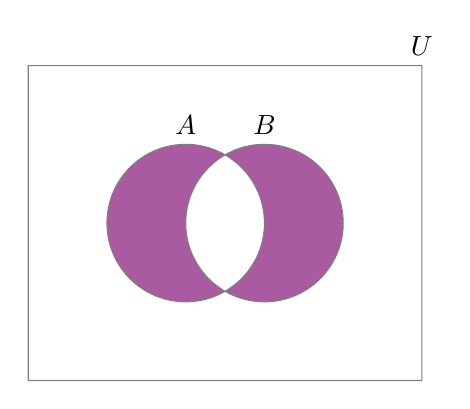
\begin{tikzpicture}[fill=zesty purple]
		% left hand
		\begin{scope}
			\clip (-2, -2) rectangle (2, 2) 
				(1, 0) circle (1);
			\fill (0, 0) circle (1);
		\end{scope}
		% right hand
		\begin{scope}
			\clip (-2, -2) rectangle (2, 2) 
				(0, 0) circle (1);
			\fill (1, 0) circle (1);
		\end{scope}
		% outline
		\draw[gray] 
			(0, 0) circle (1) 
			(0, 1)  node [text=black, above] {$A$}
			(1, 0) circle (1) 
			(1, 1)  node [text=black, above] {$B$}
			(-2, -2) rectangle 
			(3, 2) node [text=black, above] {$U$};
	\end{tikzpicture}
\end{equation*}
\end{statement}

\begin{proof}
We first draw a Venn diagram for $(A \cup B) \setminus (A \cap B)$.
Here we use orange vertical lines to shade the portion corresponding to $(A \cup B)$.
We then use blue horizontal lines to shade the portion corresponding to $(A \cap B)$.
\begin{equation*}
	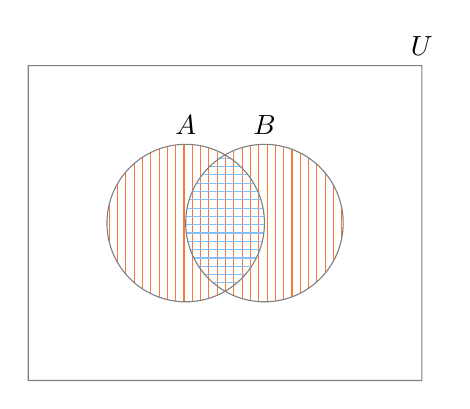
\begin{tikzpicture}
		% left hand
		\begin{scope}
			\fill[pattern color = zesty orange, pattern = vertical lines] (0, 0) circle (1);
			\fill[pattern color = zesty blue, pattern = horizontal lines] (1, 0) circle (1);
		\end{scope}
		% right hand
		\begin{scope}
			\clip (-2, -2) rectangle (2, 2) 
				(0, 0) circle (1);
			\fill[white] (1, 0) circle (1);
			\fill[pattern color = zesty orange, pattern = vertical lines] (1, 0) circle (1);
		\end{scope}
		% outline
		\draw[gray] 
			(0, 0) circle (1) 
			(0, 1)  node [text=black, above] {$A$}
			(1, 0) circle (1) 
			(1, 1)  node [text=black, above] {$B$}
			(-2, -2) rectangle 
			(3, 2) node [text=black, above] {$U$};
	\end{tikzpicture}
\end{equation*}
After removing the portion with blue shading, we are left with the following Venn diagram.
\begin{equation*}
	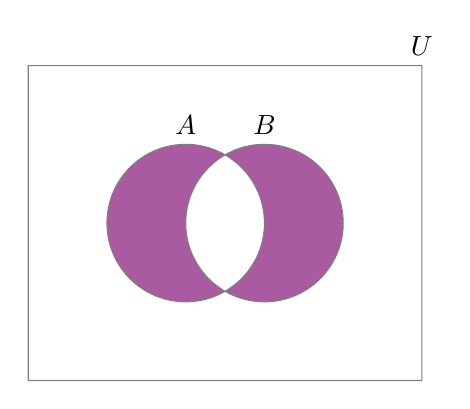
\begin{tikzpicture}[fill = zesty purple]
		% left hand
		\begin{scope}
			\clip (-2, -2) rectangle (2, 2) 
				(1, 0) circle (1);
			\fill (0, 0) circle (1);
		\end{scope}
		% right hand
		\begin{scope}
			\clip (-2, -2) rectangle (2, 2) 
				(0, 0) circle (1);
			\fill (1, 0) circle (1);
		\end{scope}
		% outline
		\draw[gray] 
			(0, 0) circle (1) 
			(0, 1)  node [text=black, above] {$A$}
			(1, 0) circle (1) 
			(1, 1)  node [text=black, above] {$B$}
			(-2, -2) rectangle 
			(3, 2) node [text=black, above] {$U$};
	\end{tikzpicture}
\end{equation*}
Next we draw a Venn diagram for $(A \setminus B) \cup (B \setminus A)$.
Here we use orange vertical lines to shade the portion corresponding to $(A \setminus B)$.
We then use blue horizontal lines to shade the portion corresponding to $(B \setminus A)$.
\begin{equation*}
	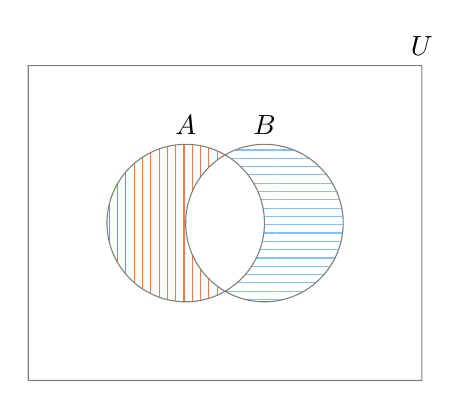
\begin{tikzpicture}
		% left hand
		\begin{scope}
			\clip (-2, -2) rectangle (2, 2) 
				(1, 0) circle (1);
			\fill[pattern color = zesty orange, pattern = vertical lines] (0, 0) circle (1);
		\end{scope}
		% right hand
		\begin{scope}
			\clip (-2, -2) rectangle (2, 2) 
				(0, 0) circle (1);
			\fill[pattern color = zesty blue, pattern = horizontal lines] (1, 0) circle (1);
		\end{scope}
		% outline
		\draw[gray] 
			(0, 0) circle (1) 
			(0, 1)  node [text=black, above] {$A$}
			(1, 0) circle (1) 
			(1, 1)  node [text=black, above] {$B$}
			(-2, -2) rectangle 
			(3, 2) node [text=black, above] {$U$};
	\end{tikzpicture}
\end{equation*}
As we can see, both Venn diagrams match the one shown in the problem statement.
\end{proof}


\begin{statement}{1.4.4}
Use Venn diagrams to verify the following identities:
\begin{enumerate}
	\item $A \setminus (A \cap B) = A \setminus B$.
	\item $A \cup (B \cap C) = (A \cup B) \cap (A \cup C)$.
\end{enumerate}
\end{statement}

\begin{proof}
\hfill
\begin{enumerate}
	\item We first draw a Venn diagram for $A  \setminus (A \cap B)$.
	Here we use orange vertical lines to shade the portion corresponding to $A$.
	We then use blue horizontal lines to shade the portion corresponding to $(A \cap B)$.
	\begin{equation*}
		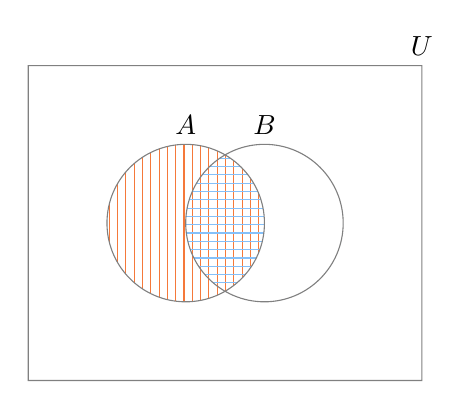
\begin{tikzpicture}
			% left hand
			\begin{scope}
				\fill[pattern color = zesty orange, pattern = vertical lines] (0, 0) circle (1);
				\fill[pattern color = zesty blue, pattern = horizontal lines] (1, 0) circle (1);
			\end{scope}
			% right hand
			\begin{scope}
				\clip (-2, -2) rectangle (2, 2) 
					(0, 0) circle (1);
				\fill[white] (1, 0) circle (1);
			\end{scope}
			% outline
			\draw[gray] 
				(0, 0) circle (1) 
				(0, 1)  node [text=black, above] {$A$}
				(1, 0) circle (1) 
				(1, 1)  node [text=black, above] {$B$}
				(-2, -2) rectangle 
				(3, 2) node [text=black, above] {$U$};
		\end{tikzpicture}
	\end{equation*}
	After removing the portion with blue shading, we are left with the following Venn diagram.
	\begin{equation*}
		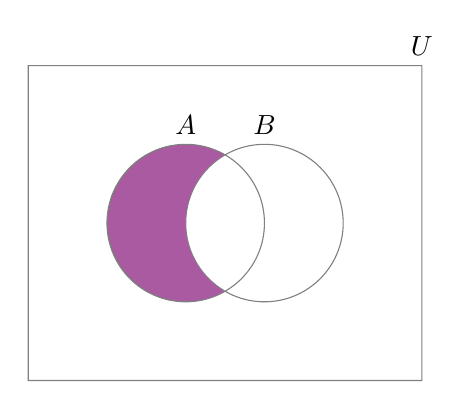
\begin{tikzpicture}[fill = zesty purple]
			% left hand
			\begin{scope}
				\clip (-2, -2) rectangle (2, 2) 
					(1, 0) circle (1);
				\fill (0, 0) circle (1);
			\end{scope}
			% outline
			\draw[gray] 
				(0, 0) circle (1) 
				(0, 1)  node [text=black, above] {$A$}
				(1, 0) circle (1) 
				(1, 1)  node [text=black, above] {$B$}
				(-2, -2) rectangle 
				(3, 2) node [text=black, above] {$U$};
		\end{tikzpicture}
	\end{equation*}
	Next we draw a Venn diagram for $A \setminus B$.
	Here we use orange vertical lines to shade the portion corresponding to $A$.
	We then use blue horizontal lines to shade the portion corresponding to $B$.
	\begin{equation*}
		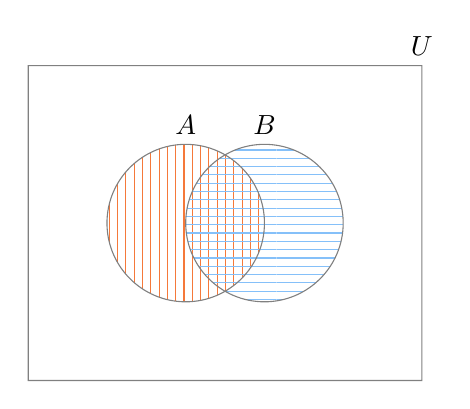
\begin{tikzpicture}
			% left hand
			\begin{scope}
				\fill[pattern color = zesty orange, pattern = vertical lines] (0, 0) circle (1);
			\end{scope}
			% right hand
			\begin{scope}
				\fill[pattern color = zesty blue, pattern = horizontal lines] (1, 0) circle (1);
			\end{scope}
			% outline
			\draw[gray] 
				(0, 0) circle (1) 
				(0, 1)  node [text=black, above] {$A$}
				(1, 0) circle (1) 
				(1, 1)  node [text=black, above] {$B$}
				(-2, -2) rectangle 
				(3, 2) node [text=black, above] {$U$};
		\end{tikzpicture}
	\end{equation*}
	After removing the part with blue shading, we are left with a Venn diagram that matches the one for $A \setminus (A \cap B)$.
	
	\item We first draw a Venn diagram for $A  \cup (B \cap C)$.
	Here we use orange vertical lines to shade the portion corresponding to $A$.
	We then use blue horizontal lines to shade the portion corresponding to $(B \cup C)$.
	\begin{equation*}
		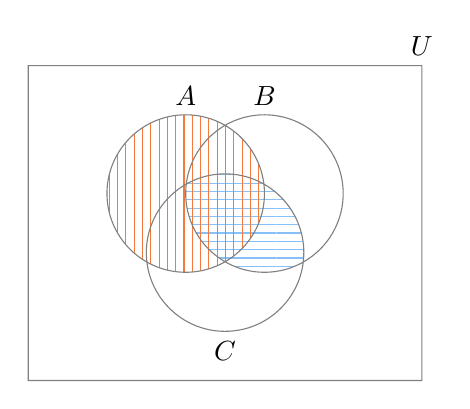
\begin{tikzpicture}
			% circle for B
			\begin{scope}
				\fill[pattern color = zesty blue, pattern = horizontal lines] (1, 0.375) circle (1);
				\clip (-2, -2) rectangle (2, 2) 
					(0.5, -0.375) circle (1);
				\fill[white] (1, 0.375) circle (1);
			\end{scope}
			% circle for A
			\begin{scope}
				\fill[pattern color = zesty orange, pattern = vertical lines] (0, 0.375) circle (1);
			\end{scope}
			% outline
			\draw[gray] 
				(0, 0.375) circle (1) 
				(0, 1.375)  node [text=black, above] {$A$}
				(1, 0.375) circle (1) 
				(1, 1.375)  node [text=black, above] {$B$}
				(0.5, -0.375) circle (1)
				(0.5, -1.375) node [text=black, below] {$C$}
				(-2, -2) rectangle 
				(3, 2) node [text=black, above] {$U$};
		\end{tikzpicture}
	\end{equation*}
	After combining the two portions of shading, we are left with the following Venn diagram.
	\begin{equation*}
		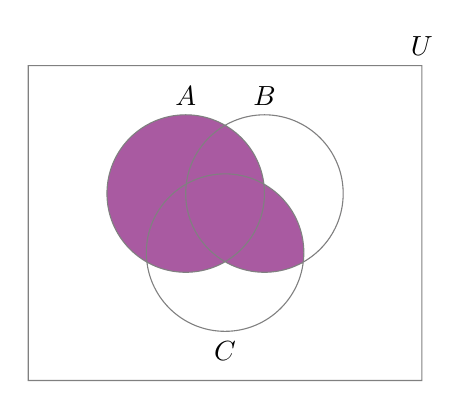
\begin{tikzpicture}[fill = zesty purple]
			% circle for B
			\begin{scope}
				\fill (1, 0.375) circle (1);
				\clip (-2, -2) rectangle (2, 2) 
					(0.5, -0.375) circle (1);
				\fill[white] (1, 0.375) circle (1);
			\end{scope}
			% circle for A
			\begin{scope}
				\fill (0, 0.375) circle (1);
			\end{scope}
			% outline
			\draw[gray] 
				(0, 0.375) circle (1) 
				(0, 1.375)  node [text=black, above] {$A$}
				(1, 0.375) circle (1) 
				(1, 1.375)  node [text=black, above] {$B$}
				(0.5, -0.375) circle (1)
				(0.5, -1.375) node [text=black, below] {$C$}
				(-2, -2) rectangle 
				(3, 2) node [text=black, above] {$U$};
		\end{tikzpicture}
	\end{equation*}
	Next we draw a Venn diagram for $(A \cup B) \cap (A \cup C)$.
	Here we use orange vertical lines to shade the portion corresponding to $A \cup B$.
	We then use blue horizontal lines to shade the portion corresponding to $A \cup C$.
	\begin{equation*}
		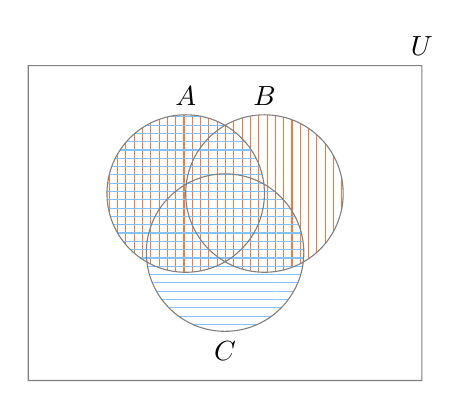
\begin{tikzpicture}
			% part for A union B
			\begin{scope}
				\fill[pattern color = zesty orange, pattern = vertical lines] (0, 0.375) circle (1);
				\fill[pattern color = zesty orange, pattern = vertical lines] (1, 0.375) circle (1);
			\end{scope}
			% part for A union C
			\begin{scope}
				\fill[pattern color = zesty blue, pattern = horizontal lines] (0, 0.375) circle (1);
				\fill[pattern color = zesty blue, pattern = horizontal lines] (0.5, -0.375) circle (1);
			\end{scope}
			% outline
			\draw[gray] 
				(0, 0.375) circle (1) 
				(0, 1.375)  node [text=black, above] {$A$}
				(1, 0.375) circle (1) 
				(1, 1.375)  node [text=black, above] {$B$}
				(0.5, -0.375) circle (1)
				(0.5, -1.375) node [text=black, below] {$C$}
				(-2, -2) rectangle 
				(3, 2) node [text=black, above] {$U$};
		\end{tikzpicture}
	\end{equation*}
	After taking only the parts with overlapping shading, we are left with a Venn diagram that matches the one for $A \cup (B \cap C)$.
\end{enumerate}
\end{proof}


\begin{statement}{1.4.5}
Verify the identities in Exercise 1.4.4 by writing out (using logical symbols) what it means for an object $x$ to be an element of each set and then using logical equivalences.
\end{statement}

\begin{proof}
For shorthand, we use lowercase letters to represent the statement that $x$ is an element of the set with the corresponding capital letter.
For example, $a$ stands for the statement $x \in A$.
\begin{enumerate}
	\item We show that $A \setminus (A \cap B) = A \setminus B$.
	\begin{align*}
		x \in A \setminus (A \cap B)
		&= a \wedge \neg (a \wedge b) \\
		&= a \wedge (\neg a \vee \neg b) \\
		&= (a \wedge \neg a) \vee (a \wedge \neg b) \\
		&= a \wedge \neg b \\
		&= x \in A \setminus B
	\end{align*}
	
	\item We show that $A \cup (B \cap C) = (A \cup B) \cap (A \cup C)$.
	\begin{align*}
		x \in A \cup (B \cap C)
		&= a \vee (b \wedge c) \\
		&= (a \vee b) \wedge (a \vee c) \\
		&= x \in (A \cup B) \cap (A \cup C)
	\end{align*}
\end{enumerate}
\end{proof}


\begin{statement}{1.4.6}
Use Venn diagrams to verify the following identities:
\begin{enumerate}
	\item $(A \cup B) \setminus C = (A \setminus C) \cup (B \setminus C)$.
	\item $A \cup (B \setminus C) = (A \cup B) \setminus (C \setminus A)$.
\end{enumerate}
\end{statement}

\begin{proof}
\hfill
\begin{enumerate}
	\item We first draw a Venn diagram for $(A \cup B) \setminus C$.
	Here we use orange vertical lines to shade the portion corresponding to $A \cup B$.
	We then use blue horizontal lines to shade the portion corresponding to $C$.
	\begin{equation*}
		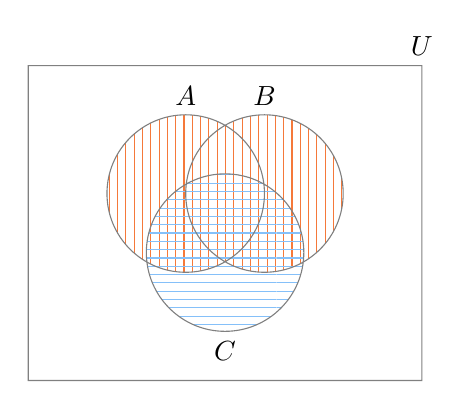
\begin{tikzpicture}
			% part for A union B
			\begin{scope}
				\fill[pattern color = zesty orange, pattern = vertical lines] (0, 0.375) circle (1);
				\fill[pattern color = zesty orange, pattern = vertical lines] (1, 0.375) circle (1);
			\end{scope}
			% part for C
			\begin{scope}
				\fill[pattern color = zesty blue, pattern = horizontal lines] (0.5, -0.375) circle (1);
			\end{scope}
			% outline
			\draw[gray] 
				(0, 0.375) circle (1) 
				(0, 1.375)  node [text=black, above] {$A$}
				(1, 0.375) circle (1) 
				(1, 1.375)  node [text=black, above] {$B$}
				(0.5, -0.375) circle (1)
				(0.5, -1.375) node [text=black, below] {$C$}
				(-2, -2) rectangle 
				(3, 2) node [text=black, above] {$U$};
		\end{tikzpicture}
	\end{equation*}
	After removing the portion with blue shading, we are left with the following Venn diagram.
	\begin{equation*}
		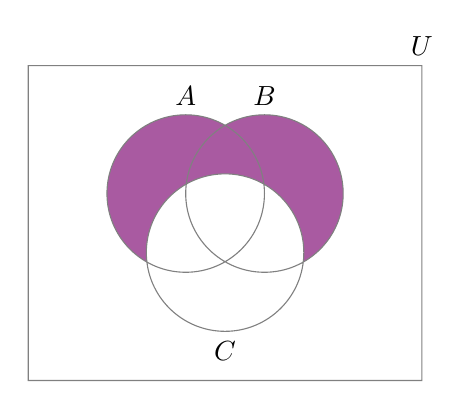
\begin{tikzpicture}
			% part for A union B
			\begin{scope}
				\fill[color = zesty purple] (0, 0.375) circle (1);
				\fill[color = zesty purple] (1, 0.375) circle (1);
			\end{scope}
			% part for C
			\begin{scope}
				\fill[color = white] (0.5, -0.375) circle (1);
			\end{scope}
			% outline
			\draw[gray] 
				(0, 0.375) circle (1) 
				(0, 1.375)  node [text=black, above] {$A$}
				(1, 0.375) circle (1) 
				(1, 1.375)  node [text=black, above] {$B$}
				(0.5, -0.375) circle (1)
				(0.5, -1.375) node [text=black, below] {$C$}
				(-2, -2) rectangle 
				(3, 2) node [text=black, above] {$U$};
		\end{tikzpicture}
	\end{equation*}
	Next we draw a Venn diagram for $(A \setminus C) \cup (B \setminus C)$.
	Here we use orange vertical lines to shade the portion corresponding to $A \setminus C$.
	We then use blue horizontal lines to shade the portion corresponding to $B \setminus C$.
	\begin{equation*}
		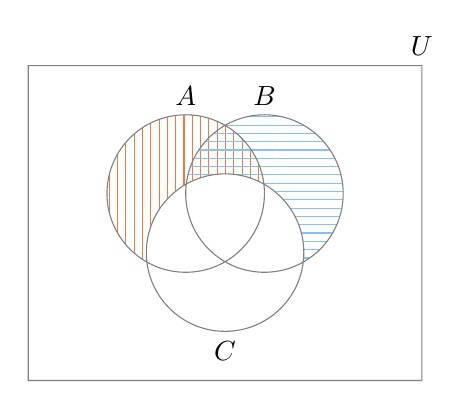
\begin{tikzpicture}
			% part for A\C
			\begin{scope}
				\clip (-2, -2) rectangle (2, 2) 
					(0.5, -0.375) circle (1);
				\fill[pattern color = zesty orange, pattern = vertical lines] (0, 0.375) circle (1);
			\end{scope}
			% part for B\C
			\begin{scope}
				\clip (-2, -2) rectangle (2, 2) 
					(0.5, -0.375) circle (1);
				\fill[pattern color = zesty blue, pattern = horizontal lines] (1, 0.375) circle (1);
			\end{scope}
			% outline
			\draw[gray] 
				(0, 0.375) circle (1) 
				(0, 1.375)  node [text=black, above] {$A$}
				(1, 0.375) circle (1) 
				(1, 1.375)  node [text=black, above] {$B$}
				(0.5, -0.375) circle (1)
				(0.5, -1.375) node [text=black, below] {$C$}
				(-2, -2) rectangle 
				(3, 2) node [text=black, above] {$U$};
		\end{tikzpicture}
	\end{equation*}
	After combining the two portions of shading, we are left with a Venn diagram that matches the one for $(A \cup B) \setminus C$.
	
	\item We first draw a Venn diagram for $A  \cup (B \setminus C)$.
	Here we use orange vertical lines to shade the portion corresponding to $A$.
	We then use blue horizontal lines to shade the portion corresponding to $(B \setminus C)$.
	\begin{equation*}	
		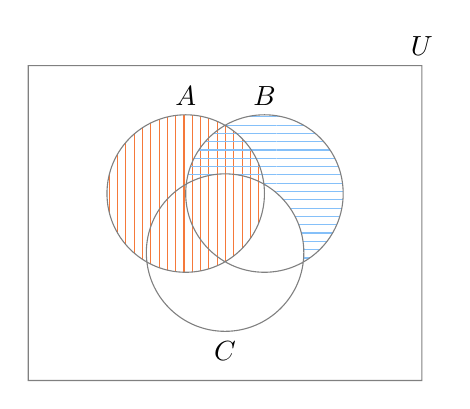
\begin{tikzpicture}
			% part for A
			\begin{scope}
				\fill[pattern color = zesty orange, pattern = vertical lines] (0, 0.375) circle (1);
			\end{scope}
			% part for B\C
			\begin{scope}
				\clip (-2, -2) rectangle (2, 2) 
					(0.5, -0.375) circle (1);
				\fill[pattern color = zesty blue, pattern = horizontal lines] (1, 0.375) circle (1);
			\end{scope}
			% outline
			\draw[gray] 
				(0, 0.375) circle (1) 
				(0, 1.375)  node [text=black, above] {$A$}
				(1, 0.375) circle (1) 
				(1, 1.375)  node [text=black, above] {$B$}
				(0.5, -0.375) circle (1)
				(0.5, -1.375) node [text=black, below] {$C$}
				(-2, -2) rectangle 
				(3, 2) node [text=black, above] {$U$};
		\end{tikzpicture}
	\end{equation*}
	After combining the two portions of shading, we are left with the following Venn diagram.
	\begin{equation*}	
		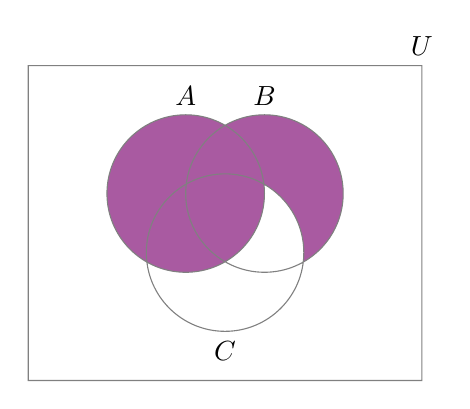
\begin{tikzpicture}[fill = zesty purple]
			% part for A
			\begin{scope}
				\fill (0, 0.375) circle (1);
			\end{scope}
			% part for B\C
			\begin{scope}
				\clip (-2, -2) rectangle (2, 2) 
					(0.5, -0.375) circle (1);
				\fill (1, 0.375) circle (1);
			\end{scope}
			% outline
			\draw[gray] 
				(0, 0.375) circle (1) 
				(0, 1.375)  node [text=black, above] {$A$}
				(1, 0.375) circle (1) 
				(1, 1.375)  node [text=black, above] {$B$}
				(0.5, -0.375) circle (1)
				(0.5, -1.375) node [text=black, below] {$C$}
				(-2, -2) rectangle 
				(3, 2) node [text=black, above] {$U$};
		\end{tikzpicture}
	\end{equation*}
	Next we draw a Venn diagram for $(A \cup B) \setminus (C \setminus A)$.
	Here we use orange vertical lines to shade the portion corresponding to $A \cup B$.
	We then use blue horizontal lines to shade the portion corresponding to $C \setminus A$.
	\begin{equation*}	
		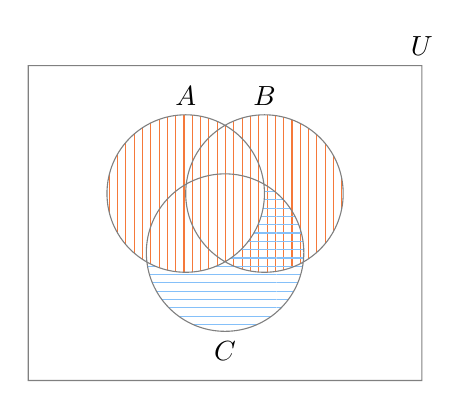
\begin{tikzpicture}
			% part for A union B
			\begin{scope}
				\fill[pattern color = zesty orange, pattern = vertical lines] (0, 0.375) circle (1);
				\fill[pattern color = zesty orange, pattern = vertical lines] (1, 0.375) circle (1);
			\end{scope}
			% part for C\A
			\begin{scope}
				\clip (-2, -2) rectangle (2, 2) 
					(0, 0.375) circle (1);
				\fill[pattern color = zesty blue, pattern = horizontal lines] (0.5, -0.375) circle (1);
			\end{scope}
			% outline
			\draw[gray] 
				(0, 0.375) circle (1) 
				(0, 1.375)  node [text=black, above] {$A$}
				(1, 0.375) circle (1) 
				(1, 1.375)  node [text=black, above] {$B$}
				(0.5, -0.375) circle (1)
				(0.5, -1.375) node [text=black, below] {$C$}
				(-2, -2) rectangle 
				(3, 2) node [text=black, above] {$U$};
		\end{tikzpicture}
	\end{equation*}
	After removing the part with blue shading, we are left with a Venn diagram that matches the one for $A \cup (B \setminus C)$.
\end{enumerate}
\end{proof}


\begin{statement}{1.4.7}
Verify the identities in Exercise 1.4.6 by writing out (using logical symbols) what it means for an object $x$ to be an element of each set and then using logical equivalences.
\end{statement}

\begin{proof}
For shorthand, we use lowercase letters to represent the statement that $x$ is an element of the set with the corresponding capital letter.
For example, $a$ stands for the statement $x \in A$.
\begin{enumerate}
	\item We show that $(A \cup B) \setminus C = (A \setminus C) \cup (B \setminus C)$.
	\begin{align*}
		x \in (A \cup B) \setminus C
		&= (a \vee b) \wedge \neg c \\
		&= (a \wedge \neg c) \vee (b \wedge \neg c) \\
		&= x \in (A \setminus C) \cup (B \setminus C)
	\end{align*}
	
	\item We show that $A \cup (B \setminus C) = (A \cup B) \setminus (C \setminus A)$.
	\begin{align*}
		x \in A \cup (B \setminus C)
		&= a \vee (b \wedge \neg c) \\
		&= (a \vee b) \wedge (a \vee \neg c) \\
		&= (a \vee b) \wedge \neg (\neg a \wedge c) \\
		&= x \in (A \cup B) \setminus (C \setminus A)
	\end{align*}
\end{enumerate}
\end{proof}


\begin{statement}{1.4.8}
Use any method you wish to verify the following identities:
\begin{enumerate}
	\item $(A \setminus B) \cap C = (A \cap C) \setminus B$.
	\item $(A \cap B) \setminus B = \varnothing$.
	\item $A \setminus (A \setminus B) = A \cap B$.
\end{enumerate}
\end{statement}

\begin{proof}
For shorthand, we use lowercase letters to represent the statement that $x$ is an element of the set with the corresponding capital letter.
For example, $a$ stands for the statement $x \in A$.
\begin{enumerate}
	\item We show that $(A \setminus B) \cap C = (A \cap C) \setminus B$.
	\begin{align*}
		x \in (A \setminus B) \cap C
		&= (a \wedge \neg b) \wedge c \\
		&= (a \wedge c) \wedge \neg b \\
		&= x \in (A \cap C) \setminus B
	\end{align*}
	
	\item We show that $(A \cap B) \setminus B = \varnothing$.
	\begin{align*}
		x \in (A \cap B) \setminus B
		&= (a \wedge b) \wedge \neg b \\
		&= a \wedge F \\
		&= F
	\end{align*}
	Since $x \in (A \cap B) \setminus B$ is always false, and therefore a contradiction, we conclude that $(A \cap B) \setminus B$ is empty.
	
	\item We show that $A \setminus (A \setminus B) = A \cap B$.
	\begin{align*}
		x \in A \setminus (A \setminus B)
		&= a \wedge \neg (a \wedge \neg b) \\
		&= a \wedge (\neg a \vee b) \\
		&= (a \wedge \neg a) \vee (a \wedge b) \\
		&= a \wedge b \\
		&= x \in A \cap B
	\end{align*}
\end{enumerate}
Of course, an alternative proof strategy would be to draw Venn diagrams to visualize the identities.
\end{proof}


\begin{statement}{1.4.9}
For each of the following sets, write out (using logical symbols) what it means for an object $x$ to be an element of the set.
Then determine which of these sets must be equal to each other by determining which statements are equivalent.
\begin{enumerate}
	\item $(A \setminus B) \setminus C$.
	\item $A \setminus (B \setminus C)$.
	\item $(A \setminus B) \cup (A \cap C)$.
	\item $(A \setminus B) \cap (A \setminus C)$.
	\item $A \setminus (B \cup C)$.
\end{enumerate}
\end{statement}

\begin{proof}
We will show the following equalities of sets.
\begin{equation*}
	(A \setminus B) \setminus C = (A \setminus B) \cap (A \setminus C) = A \setminus (B \cup C)
\end{equation*}
\begin{equation*}
	A \setminus (B \setminus C) = (A \setminus B) \cup (A \cap C)
\end{equation*}
For shorthand, we use lowercase letters to represent the statement that $x$ is an element of the set with the corresponding capital letter.
For example, $a$ stands for the statement $x \in A$.
\begin{enumerate}
	\item We show that $(A \setminus B) \setminus C = (A \setminus B) \cap (A \setminus C)$.
	\begin{align*}
		x \in (A \setminus B) \setminus C
		&= a \wedge \neg b \wedge \neg c \\
		&= (a \wedge \neg b) \wedge (a \wedge \neg c) \\
		&= x \in (A \setminus B) \cap (A \setminus C)
	\end{align*}
	
	\item We show that $(A \setminus B) \setminus C = A \setminus (B \cup C)$
	\begin{align*}
		x \in (A \setminus B) \setminus C
		&= a \wedge \neg b \wedge \neg c \\
		&= a \wedge \neg (b \vee c) \\
		&= x \in A \setminus (B \cup C)
	\end{align*}
	
	\item We show that $A \setminus (B \setminus C) = (A \setminus B) \cup (A \cap C)$.
	\begin{align*}
		x \in A \setminus (B \setminus C)
		&= a \wedge \neg (b \wedge \neg c) \\
		&= a \wedge (\neg b \vee c) \\
		&= (a \wedge \neg b) \vee (a \wedge c) \\
		&= x \in (A \setminus B) \cup (A \cap C)
	\end{align*}
\end{enumerate}
\end{proof}


\begin{statement}{1.4.10}
It was shown in this section that for any sets $A$ and $B$, $(A \cup B) \setminus B \subseteq A$.
\begin{enumerate}
	\item Give an example of two sets $A$ and $B$ for which $(A \cup B) \setminus B = A$.
	\item Show that for all sets $A$ and $B$, $(A \cup B) \setminus B = A \setminus B$.
\end{enumerate}
\end{statement}

\begin{proof}
\hfill
\begin{enumerate}
	\item Consider $A = \{ 1, 2, 3 \}$ and $B = \{ 4, 5, 6 \}$.
	In this situation $A \cup B = \{ 1, 2, 3, 4, 5, 6 \}$, so then $(A \cup B) \setminus B = \{ 1, 2, 3 \} = A$.
	\item For shorthand, we use lowercase letters to represent the statement that $x$ is an element of the set with the corresponding capital letter.
	For example, $a$ stands for the statement $x \in A$.
	We now show that $(A \cup B) \setminus B = A \setminus B$.
	\begin{align*}
		x \in (A \cup B) \setminus B
		&= (a \vee b) \wedge \neg b \\
		&= (a \wedge \neg b) \vee (b \wedge \neg b) \\
		&= (a \wedge \neg b) \\
		&= x \in A \setminus B
	\end{align*}
\end{enumerate}
\end{proof}


\begin{statement}{1.4.11}
Suppose $A$ and $B$ are sets.
Is it necessarily true that $(A \setminus B) \cup B = A$?
If not, is one of these sets necessarily a subset of the other?
Is $(A \setminus B) \cup B$ always equal to either $A \setminus B$ or $A \cup B$?
\end{statement}

\begin{proof}
$(A \setminus B) \cup B$ is not necessarily equal to $A$.
For example, consider the sets $A = \{ 1, 2, 3 \}$ and $B = \{ 4, 5, 6 \}$.
In this case $(A \setminus B) \cup B = \{ 1, 2, 3, 4, 5, 6 \} = A \cup B$.
In fact, $(A \setminus B) \cup B = A \cup B$ in general.
To see this, let $a$ stand for $x \in A$ and let $b$ stand for $x \in B$.
Then $x \in (A \setminus B) \cup B$ has the logical form $(a \wedge \neg b) \vee b$.
This is equivalent to $(a \vee b) \wedge (\neg b \vee b)$, which in turn is equivalent to $a \vee b$.
Thus, we conclude that $(A \setminus B) \cup B = A \cup B$.
Knowing this also tells us that $A \subseteq A \cup B = (A \setminus B) \cup B$
\end{proof}


\begin{statement}{1.4.12}
It is claimed in this section that you cannot make a Venn diagram for four sets using overlapping circles.
\begin{enumerate}
	\item What's wrong with the following diagram?
	\emph{(Hint: Where's the set $(A \cap D) \setminus (B \cup C)$?)}
	\begin{equation*}
		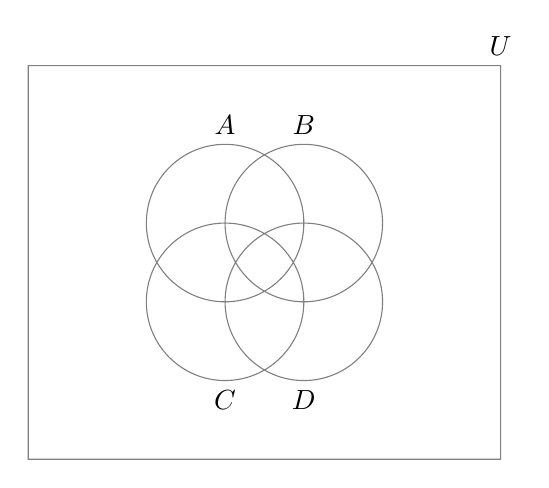
\begin{tikzpicture}
			% outline
			\draw[gray]
				(0, 0.5) circle (1) 
				(0, 1.5)  node [text = black, above] {$A$}
				(1, 0.5) circle (1) 
				(1, 1.5)  node [text = black, above] {$B$}
				(0, -0.5) circle (1) 
				(0, -1.5)  node [text = black, below] {$C$}
				(1, -0.5) circle (1) 
				(1, -1.5)  node [text = black, below] {$D$}
				(-2.5, -2.5) rectangle 
				(3.5, 2.5) node [text = black, above] {$U$};
		\end{tikzpicture}
	\end{equation*}
	
	\item Can you make a Venn diagram for four sets using shapes other than circles?
\end{enumerate}
\end{statement}

\begin{proof}
\hfill
\begin{enumerate}
	\item Following the hint, we try to find the set $(A \cap D) \setminus (B \cup C)$.
	We use orange vertical lines to shade the portion corresponding to $A \cap D$.
	We then use blue horizontal lines to shade the portion corresponding to $B \cup C$.
	\begin{equation*}
		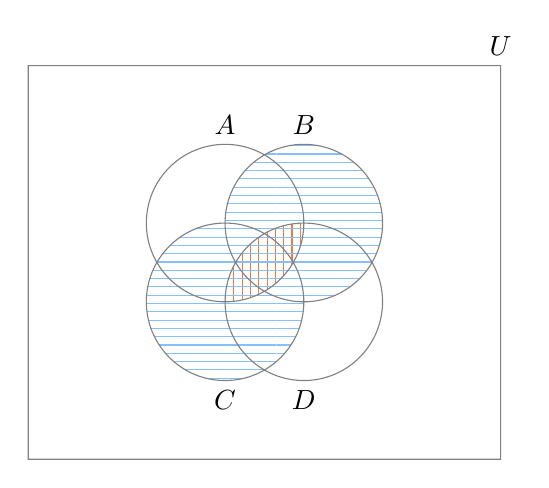
\begin{tikzpicture}
			% Part for A intersect D
			\begin{scope}
				\fill[pattern color = zesty orange, pattern = vertical lines] (0, 0.5) circle (1);
				\clip (-2.5, -2.5) rectangle (2.5, 2.5) 
					(1, -0.5) circle (1);
				\fill[white] (0, 0.5) circle (1);
			\end{scope}
			% Part for B union C
			\begin{scope}
				\fill[pattern color = zesty blue, pattern = horizontal lines] (1, 0.5) circle (1);
				\fill[pattern color = zesty blue, pattern = horizontal lines] (0, -0.5) circle (1);
			\end{scope}
			% outline
			\draw[gray]
				(0, 0.5) circle (1) 
				(0, 1.5)  node [text = black, above] {$A$}
				(1, 0.5) circle (1) 
				(1, 1.5)  node [text = black, above] {$B$}
				(0, -0.5) circle (1) 
				(0, -1.5)  node [text = black, below] {$C$}
				(1, -0.5) circle (1) 
				(1, -1.5)  node [text = black, below] {$D$}
				(-2.5, -2.5) rectangle 
				(3.5, 2.5) node [text = black, above] {$U$};
		\end{tikzpicture}
	\end{equation*}
	As we can see, in this diagram the blue portion completely overlaps the orange.
	This means that even though the set $(A \cap D) \setminus (B \cup C)$ may be nonempty, it is not present in the diagram.
	
	\item One way to make a proper Venn diagram for four sets is as follows.
	\begin{equation*}
		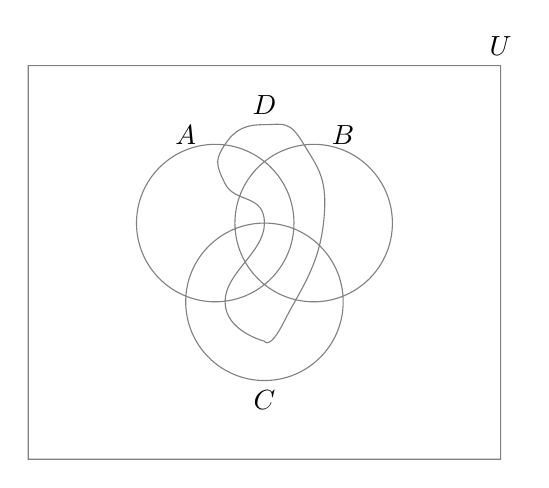
\begin{tikzpicture}
			% outline
			\draw[gray]
				(-0.125, 0.5) circle (1) 
				(-0.5, 1.375)  node [text=black, above] {$A$}
				(1.125, 0.5) circle (1) 
				(1.5, 1.375)  node [text=black, above] {$B$}
				(0.5, -0.5) circle (1)
				(0.5, -1.5) node [text=black, below] {$C$}
				% If you feel up to do so later, try to come back and clean this up
				plot[smooth, tension=.9] 
					coordinates {(0.5, -1) (0, -0.5) (0.5, 0.5) (0, 1) (0, 1.5) (0.5, 1.75)
					(1, 1.5) (1.25, 0.5) (0.75, -0.75) (0.5, -1)}
				(0.5, 1.75) node[text = black, above] {$D$}
				(-2.5, -2.5) rectangle 
				(3.5, 2.5) node [text=black, above] {$U$};
		\end{tikzpicture}
	\end{equation*}
\end{enumerate}
\end{proof}


\begin{statement}{1.4.13}
\begin{enumerate}
	\item Make Venn diagrams for the sets $(A \cup B) \setminus C$ and $A \cup (B \setminus C)$.
	What can you conclude about whether one of these sets is necessarily a subset of the other?
	
	\item Give an example of sets $A$, $B$, and $C$ for which $(A \cup B) \setminus C \neq A \cup (B \setminus C)$.
\end{enumerate}
\end{statement}

\begin{proof}
\hfill
\begin{enumerate}
	\item We saw in Exercise 1.4.6 that a Venn diagram for for $(A \cup B) \setminus C$ was a follows.
	\begin{equation*}
		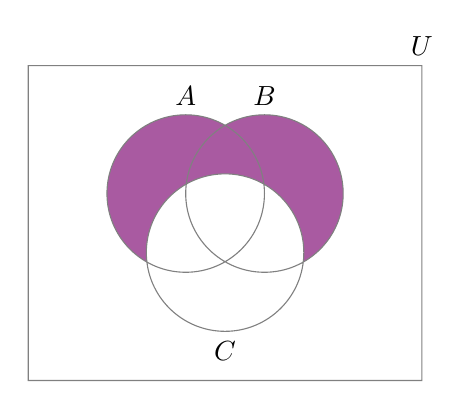
\begin{tikzpicture}
			% part for A union B
			\begin{scope}
				\fill[color = zesty purple] (0, 0.375) circle (1);
				\fill[color = zesty purple] (1, 0.375) circle (1);
			\end{scope}
			% part for C
			\begin{scope}
				\fill[color = white] (0.5, -0.375) circle (1);
			\end{scope}
			% outline
			\draw[gray] 
				(0, 0.375) circle (1) 
				(0, 1.375)  node [text=black, above] {$A$}
				(1, 0.375) circle (1) 
				(1, 1.375)  node [text=black, above] {$B$}
				(0.5, -0.375) circle (1)
				(0.5, -1.375) node [text=black, below] {$C$}
				(-2, -2) rectangle 
				(3, 2) node [text=black, above] {$U$};
		\end{tikzpicture}
	\end{equation*}
	In the same exercise, we also saw that a Venn diagram for $A \cup (B \setminus C)$ was as follows.
	\begin{equation*}	
		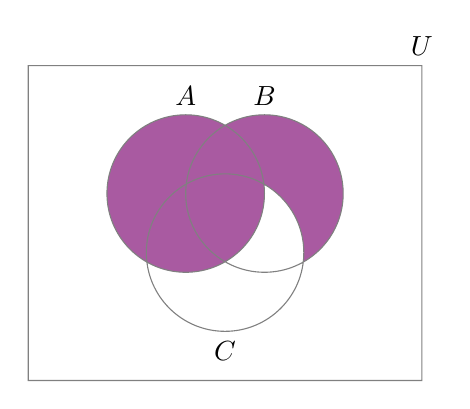
\begin{tikzpicture}[fill = zesty purple]
			% part for A
			\begin{scope}
				\fill (0, 0.375) circle (1);
			\end{scope}
			% part for B\C
			\begin{scope}
				\clip (-2, -2) rectangle (2, 2) 
					(0.5, -0.375) circle (1);
				\fill (1, 0.375) circle (1);
			\end{scope}
			% outline
			\draw[gray] 
				(0, 0.375) circle (1) 
				(0, 1.375)  node [text=black, above] {$A$}
				(1, 0.375) circle (1) 
				(1, 1.375)  node [text=black, above] {$B$}
				(0.5, -0.375) circle (1)
				(0.5, -1.375) node [text=black, below] {$C$}
				(-2, -2) rectangle 
				(3, 2) node [text=black, above] {$U$};
		\end{tikzpicture}
	\end{equation*}
	From these two Venn diagrams, we can conclude that $(A \cup B) \setminus C \subseteq A \cup (B \setminus C)$.
	
	\item Consider the sets $A = \{ 1, 2, 3 \}$, $B = \{ 4, 5, 6 \}$, and $C = \{ 3, 4 \}$.
	With these three sets, $(A \cup B) \setminus C = \{ 1, 2, 5, 6 \}$ while $A \cup (B \setminus C) = \{ 1, 2, 3, 5, 6 \}$.
	This example shows us that $(A \cup B) \setminus C$ and $A \cup (B \setminus C)$ need not be equal.
\end{enumerate}
\end{proof}


\begin{statement}{1.4.14}
Use Venn diagrams to show that the associative law holds for symmetric difference;
that is, for any sets $A$, $B$, and $C$, $A \bigtriangleup (B \bigtriangleup C) = (A \bigtriangleup B) \bigtriangleup C$.
\end{statement}

\begin{proof}
We first draw a Venn diagram for $A  \bigtriangleup (B \bigtriangleup C)$.
Here we use orange vertical lines to shade the portion corresponding to $A$.
We then use blue horizontal lines to shade the portion corresponding to $B \bigtriangleup C$.
\begin{equation*}	
	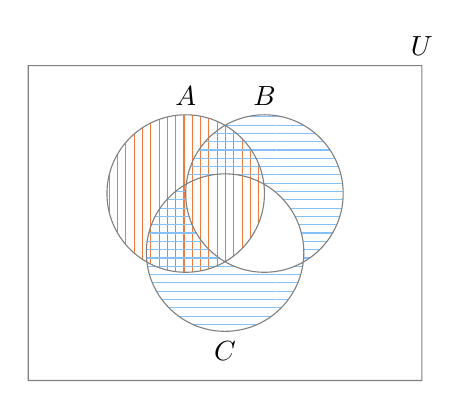
\begin{tikzpicture}
		% part for A
		\begin{scope}
			\fill[pattern color = zesty orange, pattern = vertical lines] (0, 0.375) circle (1);
		\end{scope}
		% part for B symmetric difference C
		\begin{scope}
			\clip (-2, -2) rectangle (2, 2) 
				(0.5, -0.375) circle (1);
			\fill[pattern color = zesty blue, pattern = horizontal lines] (1, 0.375) circle (1);
		\end{scope}
		\begin{scope}
			\clip (-2, -2) rectangle (2, 2) 
				(1, 0.375) circle (1);
			\fill[pattern color = zesty blue, pattern = horizontal lines] (0.5, -0.375) circle (1);
		\end{scope}
		% outline
		\draw[gray] 
			(0, 0.375) circle (1) 
			(0, 1.375)  node [text=black, above] {$A$}
			(1, 0.375) circle (1) 
			(1, 1.375)  node [text=black, above] {$B$}
			(0.5, -0.375) circle (1)
			(0.5, -1.375) node [text=black, below] {$C$}
			(-2, -2) rectangle 
			(3, 2) node [text=black, above] {$U$};
	\end{tikzpicture}
\end{equation*}
Removing the areas with overlapping shading, we are left with the following Venn diagram.
\begin{equation*}	
	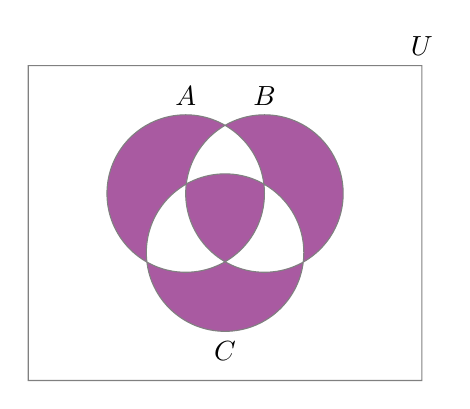
\begin{tikzpicture}[fill = zesty purple]
		% part for A
		\begin{scope}
			\fill (0, 0.375) circle (1);
		\end{scope}
		% part for B
		\begin{scope}
			\clip (-2, -2) rectangle (2, 2) 
				(0.5, -0.375) circle (1);
			\fill[white] (1, 0.375) circle (1);
			\clip (-2, -2) rectangle (2, 2) 
				(0, 0.375) circle (1)
				(0.5, -0.375) circle (1);
			\fill (1, 0.375) circle (1);
		\end{scope}
		% part for C
		\begin{scope}
			\clip (-2, -2) rectangle (2, 2) 
				(1, 0.375) circle (1);
			\fill[white] (0.5, -0.375) circle (1);
			\clip (-2, -2) rectangle (2, 2) 
				(0, 0.375) circle (1)
				(1, 0.375) circle (1);
			\fill (0.5, -0.375) circle (1);
		\end{scope}
		% outline
		\draw[gray] 
			(0, 0.375) circle (1) 
			(0, 1.375)  node [text=black, above] {$A$}
			(1, 0.375) circle (1) 
			(1, 1.375)  node [text=black, above] {$B$}
			(0.5, -0.375) circle (1)
			(0.5, -1.375) node [text=black, below] {$C$}
			(-2, -2) rectangle 
			(3, 2) node [text=black, above] {$U$};
	\end{tikzpicture}
\end{equation*}
Next we draw a Venn diagram for $(A  \bigtriangleup B) \bigtriangleup C$.
Here we use orange vertical lines to shade the portion corresponding to $A \bigtriangleup B$.
We then use blue horizontal lines to shade the portion corresponding to $C$.
\begin{equation*}	
	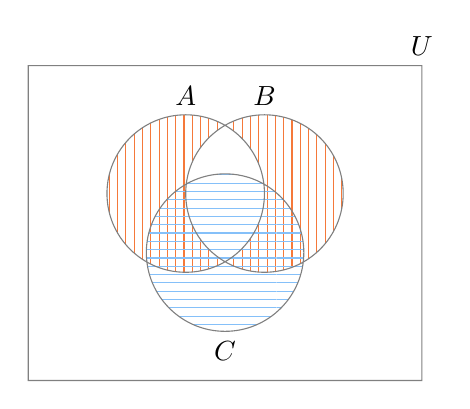
\begin{tikzpicture}
		% part for A symmetric difference B
		\begin{scope}
			\clip (-2, -2) rectangle (2, 2) 
				(1, 0.375) circle (1);
			\fill[pattern color = zesty orange, pattern = vertical lines] (0, 0.375) circle (1);
		\end{scope}
		\begin{scope}
			\clip (-2, -2) rectangle (2, 2) 
				(0, 0.375) circle (1);
			\fill[pattern color = zesty orange, pattern = vertical lines] (1, 0.375) circle (1);
		\end{scope}
		% part for C
		\begin{scope}
			\fill[pattern color = zesty blue, pattern = horizontal lines] (0.5, -0.375) circle (1);
		\end{scope}
		% outline
		\draw[gray] 
			(0, 0.375) circle (1) 
			(0, 1.375)  node [text=black, above] {$A$}
			(1, 0.375) circle (1) 
			(1, 1.375)  node [text=black, above] {$B$}
			(0.5, -0.375) circle (1)
			(0.5, -1.375) node [text=black, below] {$C$}
			(-2, -2) rectangle 
			(3, 2) node [text=black, above] {$U$};
	\end{tikzpicture}
\end{equation*}
Removing the areas with overlapping shading gives us a Venn diagram that matches the one for $A \bigtriangleup (B \bigtriangleup C)$.
\end{proof}


\begin{statement}{1.4.15}
Use any method you wish to verify the following identities:
\begin{enumerate}
	\item $(A \bigtriangleup B) \cup C = (A \cup C) \bigtriangleup (B \setminus C)$.
	\item $(A \bigtriangleup B) \cap C = (A \cap C) \bigtriangleup (B \cap C)$.
	\item $(A \bigtriangleup B) \setminus C = (A \setminus C) \bigtriangleup (B \setminus C)$.
\end{enumerate}
\end{statement}

\begin{proof}
For shorthand, we use lowercase letters to represent the statement that $x$ is an element of the set with the corresponding capital letter.
For example, $a$ stands for the statement $x \in A$.
\begin{enumerate}
	\item We first note that $(A \cup C) \bigtriangleup (B \setminus C) = [(A \cup C) \cup (B \setminus C)] \setminus [(A \cup C) \cap (B \setminus C)]$.
	The logical form for $x \in (A \cup C) \cup (B \setminus C)$ is
	\begin{equation*}
		(a \vee c) \vee (b \wedge \neg c)
		= (a \vee b \vee c) \wedge (a \vee c \vee \neg c) 
		= a \vee b \vee c.
	\end{equation*}
	The logical form for $x \in (A \cup C) \cap (B \setminus C)$ is
	\begin{equation*}
		(a \vee c) \wedge (b \wedge \neg c)
		= [(a \wedge \neg c) \vee (c \wedge \neg c)] \wedge b
		= a \wedge b \wedge \neg c.
	\end{equation*}
	These two give us the logical form for $x \in [(A \cup C) \cup (B \setminus C)] \setminus [(A \cup C) \cap (B \setminus C)]$.
	\begin{align*}
		(a \vee b \vee c) \wedge \neg (a \wedge b \wedge \neg c)
		&= [(a \vee b) \vee c] \wedge [\neg (a \wedge b) \vee c] \\
		&= [(a \vee b) \wedge \neg (a \wedge b)] \vee c \\
		&= x \in (A \bigtriangleup B) \cup C
	\end{align*}
	Thus, we conclude that $(A \bigtriangleup B) \cup C = (A \cup C) \bigtriangleup (B \setminus C)$.
	
	\item We first note that $(A \cap C) \bigtriangleup (B \cap C) = [(A \cap C) \cup (B \cap C)] \setminus [(A \cap C) \cap (B \cap C)]$.
	The logical form for $x \in (A \cap C) \cup (B \cap C)$ is
	\begin{equation*}
		(a \wedge c) \vee (b \wedge c)
		= (a \vee b) \wedge c.
	\end{equation*}
	The logical form for $x \in (A \cap C) \cap (B \cap C)$ is
	\begin{equation*}
		(a \wedge c) \wedge (b \wedge c)
		= a \wedge b \wedge c.
	\end{equation*}
	These two give us the logical form for $x \in  [(A \cap C) \cup (B \cap C)] \setminus [(A \cap C) \cap (B \cap C)]$.
	\begin{align*}
		[(a \vee b) \wedge c] \wedge \neg (a \wedge b \wedge c)
		&= [(a \vee b) \wedge c] \wedge [\neg (a \wedge b) \vee \neg c] \\
		&= [(a \vee b) \wedge \neg (a \wedge b) \wedge c] \vee [(a \vee b) \wedge c \wedge \neg c] \\
		&= [(a \vee b) \wedge \neg (a \wedge b)] \wedge c \\
		&= x \in (A \bigtriangleup B) \cap C
	\end{align*}
	Thus, we conclude that $(A \bigtriangleup B) \cap C = (A \cap C) \bigtriangleup (B \cap C)$.
	
	\item We first note that $(A \setminus C) \bigtriangleup (B \setminus C) = [(A \setminus C) \cup (B \setminus C)] \setminus [(A \setminus C) \cap (B \setminus C)]$.
	The logical form for $x \in (A \setminus C) \cup (B \setminus C)$ is
	\begin{equation*}
		(a \wedge \neg c) \vee (b \wedge \neg c)
		= (a \vee b) \wedge \neg c.
	\end{equation*}
	The logical form for $x \in (A \setminus C) \cap (B \setminus C)$ is
	\begin{equation*}
		(a \wedge \neg c) \wedge (b \wedge \neg c)
		= a \wedge b \wedge \neg c.
	\end{equation*}
	These two give us the logical form for $x \in   [(A \setminus C) \cup (B \setminus C)] \setminus [(A \setminus C) \cap (B \setminus C)]$.
	\begin{align*}
		[(a \vee b) \wedge \neg c] \wedge \neg (a \wedge b \wedge \neg c)
		&= [(a \vee b) \wedge \neg c] \wedge [\neg (a \wedge b) \vee c] \\
		&= [(a \vee b) \wedge \neg (a \wedge b) \wedge \neg c] \vee [(a \vee b) \wedge \neg c \wedge c] \\
		&= [(a \vee b) \wedge \neg (a \wedge b)] \wedge \neg c \\
		&= x \in (A \bigtriangleup B) \setminus C
	\end{align*}
	Thus, we conclude that $(A \bigtriangleup B) \setminus C = (A \setminus C) \bigtriangleup (B \setminus C)$.
\end{enumerate}
Of course, an alternative proof strategy would be to draw Venn diagrams to visualize the identities.
\end{proof}


\begin{statement}{1.4.16}
Use any method you wish to verify the following identities:
\begin{enumerate}
	\item $(A \cup B) \bigtriangleup C = (A \bigtriangleup C) \bigtriangleup (B \setminus A)$.
	\item $(A \cap B) \bigtriangleup C = (A \bigtriangleup C) \bigtriangleup (A \setminus B)$.
	\item $(A \setminus B) \bigtriangleup C = (A \bigtriangleup C) \bigtriangleup (A \cap B)$.
\end{enumerate}
\end{statement}

\begin{proof}
For shorthand, we use lowercase letters to represent the statement that $x$ is an element of the set with the corresponding capital letter.
For example, $a$ stands for the statement $x \in A$.
\begin{enumerate}
	\item We first note that $(A \bigtriangleup C) \bigtriangleup (B \setminus A) = [(A \bigtriangleup C) \cup (B \setminus A)] \setminus [(A \bigtriangleup C) \cap (B \setminus A)]$.
	The logical form for $x \in (A \bigtriangleup C) \cup (B \setminus A) = (A \setminus C) \cup (C \setminus A) \cup (B \setminus A)$ is
	\begin{equation*}
		(a \wedge \neg c) \vee (\neg a \wedge c) \vee (\neg a \wedge b).
	\end{equation*}
	The logical form for $x \in (A \bigtriangleup C) \cap (B \setminus A) = [(A \cup C) \setminus (A \cap C)] \cap (B \setminus A)$ is
	\begin{equation*}
		(a \vee c) \wedge \neg (a \wedge c) \wedge (\neg a \wedge b).
	\end{equation*}
	These two give us the logical form for $x \in [(A \bigtriangleup C) \cup (B \setminus A)] \setminus [(A \bigtriangleup C) \cap (B \setminus A)]$.
	\begin{equation*}
		[(a \wedge \neg c) \vee (\neg a \wedge c) \vee (\neg a \wedge b)]
		\wedge [(\neg a \wedge \neg c) \vee (a \wedge c) \vee (a \vee \neg b)].
	\end{equation*}
	Expanding this out gives us the following terms.
	\begin{align*}
		& (a \wedge \neg c) \wedge (\neg a \wedge \neg c) = a \wedge \neg a \wedge \neg c = F \\
		& (a \wedge \neg c) \wedge (a \wedge c) = a \wedge \neg c \wedge c = F \\
		& (a \wedge \neg c) \wedge (a \vee \neg b) 
			= (a \wedge \neg c) \vee (a \wedge \neg b \wedge \neg c) \\
		& (\neg a \wedge c) \wedge (\neg a \wedge \neg c) = \neg a \wedge c \wedge \neg c = F \\
		& (\neg a \wedge c) \wedge (a \wedge c) = \neg a \wedge a \wedge c = F \\
		& (\neg a \wedge c) \wedge (a \wedge \neg b) 
			= (\neg a \wedge a \wedge c) \vee (\neg a \wedge \neg b \wedge c) 
			= \neg a \wedge \neg b \wedge c \\
		& (\neg a \wedge b) \wedge (\neg a \wedge \neg c) = \neg a \wedge b \wedge \neg c \\
		& (\neg a \wedge b) \wedge (a \wedge c) = \neg a \wedge a \wedge b \wedge c = F \\
		& (\neg a \wedge b) \wedge (a \vee \neg b) 
			= (\neg a \wedge b) \wedge \neg (\neg a \wedge b) = F
	\end{align*}
	Now we combine the terms, using the fact that $P \vee (\text{a contradiction}) = P$.
	\begin{align*}
		& (a \wedge \neg c) \vee (a \wedge \neg b \wedge \neg c)
			\vee (\neg a \wedge \neg b \wedge c) \vee (\neg a \wedge b \wedge \neg c) \\
		&= [[a \vee (a \wedge \neg b) \vee (\neg a \wedge b)] \wedge \neg c]
			\vee [\neg (a \vee b) \wedge c] \\
		&= [(a \vee b) \wedge \neg c] \vee [\neg (a \vee b) \wedge c] \\
		&= x \in (A \cup B) \bigtriangleup C
	\end{align*}
	Thus, we conclude that $(A \cup B) \bigtriangleup C = (A \bigtriangleup C) \bigtriangleup (B \setminus A)$.
	
	\item We first note that $(A \bigtriangleup C) \bigtriangleup (A \setminus B) = [(A \bigtriangleup C) \cup (A \setminus B)] \setminus [(A \bigtriangleup C) \cap (A \setminus B)]$.
	The logical form for $x \in (A \bigtriangleup C) \cup (A \setminus B) = (A \setminus C) \cup (C \setminus A) \cup (A \setminus B)$ is
	\begin{equation*}
		(a \wedge \neg c) \vee (\neg a \wedge c) \vee (a \wedge \neg b).
	\end{equation*}
	The logical form for $x \in (A \bigtriangleup C) \cap (A \setminus B) = [(A \cup C) \setminus (A \cap C)] \cap (A \setminus B)$ is
	\begin{equation*}
		(a \vee c) \wedge \neg (a \wedge c) \wedge (a \wedge \neg b).
	\end{equation*}
	These two give us the logical form for $x \in [(A \bigtriangleup C) \cup (A \setminus B)] \setminus [(A \bigtriangleup C) \cap (A \setminus B)]$.
	\begin{equation*}
		[(a \wedge \neg c) \vee (\neg a \wedge c) \vee (a \wedge \neg b)]
		\wedge [(\neg a \wedge \neg c) \vee (a \wedge c) \vee (\neg a \vee b)].
	\end{equation*}
	Expanding this out gives us the following terms.
	\begin{align*}
		& (a \wedge \neg c) \wedge (\neg a \wedge \neg c) = a \wedge \neg a \wedge \neg c = F \\
		& (a \wedge \neg c) \wedge (a \wedge c) = a \wedge \neg c \wedge c = F \\
		& (a \wedge \neg c) \wedge (\neg a \vee b) 
			= (a \wedge \neg a \wedge \neg c) \vee (a \wedge b \wedge \neg c)
			= a \wedge b \wedge \neg c \\
		& (\neg a \wedge c) \wedge (\neg a \wedge \neg c) = \neg a \wedge c \wedge \neg c = F \\
		& (\neg a \wedge c) \wedge (a \wedge c) = \neg a \wedge a \wedge c = F \\
		& (\neg a \wedge c) \wedge (\neg a \wedge b) 
			= (\neg a \wedge c) \vee (\neg a \wedge b \wedge c) \\
		& (a \wedge \neg b) \wedge (\neg a \wedge \neg c) 
		= a \wedge \neg a \wedge \neg b \wedge \neg c = F \\
		& (a \wedge \neg b) \wedge (a \wedge c) = a \wedge \neg b \wedge c \\
		& (a \wedge \neg b) \wedge (\neg a \vee b) 
			= (a \wedge \neg b) \wedge \neg (a \wedge \neg b) = F
	\end{align*}
	Now we combine the terms, using the fact that $P \vee (\text{a contradiction}) = P$.
	\begin{align*}
		& (a \wedge b \wedge \neg c) \vee (\neg a \wedge c)
			\vee (\neg a \wedge b \wedge c) \vee (a \wedge \neg b \wedge c) \\
		&= [(a \wedge b) \wedge \neg c]
			\vee [[\neg a \vee (\neg a \wedge b) \vee (a \wedge \neg b)] \wedge c] \\
		&= [(a \wedge b) \wedge \neg c] \vee [(\neg a \vee \neg b) \wedge c] \\
		&= [(a \wedge b) \wedge \neg c] \vee [\neg (a \wedge b) \wedge c] \\
		&= x \in (A \cap B) \bigtriangleup C
	\end{align*}
	Thus, we conclude that $(A \cap B) \bigtriangleup C = (A \bigtriangleup C) \bigtriangleup (A \setminus B)$.
	
	\item We first note that $(A \bigtriangleup C) \bigtriangleup (A \cap B) = [(A \bigtriangleup C) \cup (A \cap B)] \setminus [(A \bigtriangleup C) \cap (A \cap B)]$.
	The logical form for $x \in (A \bigtriangleup C) \cup (A \cap B) = (A \setminus C) \cup (C \setminus A) \cup (A \cap B)$ is
	\begin{equation*}
		(a \wedge \neg c) \vee (\neg a \wedge c) \vee (a \wedge b).
	\end{equation*}
	The logical form for $x \in (A \bigtriangleup C) \cap (A \cap B) = [(A \cup C) \setminus (A \cap C)] \cap (A \cap B)$ is
	\begin{equation*}
		(a \vee c) \wedge \neg (a \wedge c) \wedge (a \wedge b).
	\end{equation*}
	These two give us the logical form for $x \in [(A \bigtriangleup C) \cup (A \cap B)] \setminus [(A \bigtriangleup C) \cap (A \cap B)]$.
	\begin{equation*}
		[(a \wedge \neg c) \vee (\neg a \wedge c) \vee (a \wedge b)]
		\wedge [(\neg a \wedge \neg c) \vee (a \wedge c) \vee (\neg a \vee \neg b)].
	\end{equation*}
	Expanding this out gives us the following terms.
	\begin{align*}
		& (a \wedge \neg c) \wedge (\neg a \wedge \neg c) = a \wedge \neg a \wedge \neg c = F \\
		& (a \wedge \neg c) \wedge (a \wedge c) = a \wedge \neg c \wedge c = F \\
		& (a \wedge \neg c) \wedge (\neg a \vee \neg b) 
			= (a \wedge \neg a \wedge \neg c) \vee (a \wedge \neg b \wedge \neg c)
			= a \wedge \neg b \wedge \neg c \\
		& (\neg a \wedge c) \wedge (\neg a \wedge \neg c) = \neg a \wedge c \wedge \neg c = F \\
		& (\neg a \wedge c) \wedge (a \wedge c) = \neg a \wedge a \wedge c = F \\
		& (\neg a \wedge c) \wedge (\neg a \wedge \neg b) 
			= (\neg a \wedge c) \vee (\neg a \wedge \neg b \wedge c) \\
		& (a \wedge b) \wedge (\neg a \wedge \neg c) 
		= a \wedge \neg a \wedge b \wedge \neg c = F \\
		& (a \wedge b) \wedge (a \wedge c) = a \wedge b \wedge c \\
		& (a \wedge b) \wedge (\neg a \vee \neg b) 
			= (a \wedge b) \wedge \neg (a \wedge b) = F
	\end{align*}
	Now we combine the terms, using the fact that $P \vee (\text{a contradiction}) = P$.
	\begin{align*}
		& (a \wedge \neg b \wedge \neg c) \vee (\neg a \wedge c)
			\vee (\neg a \wedge \neg b \wedge c) \vee (a \wedge b \wedge c) \\
		&= [(a \wedge \neg b) \wedge \neg c]
			\vee [[\neg a \vee (\neg a \wedge \neg b) \vee (a \wedge b)] \wedge c] \\
		&= [(a \wedge \neg b) \wedge \neg c] \vee [(\neg a \vee b) \wedge c] \\
		&= [(a \wedge \neg b) \wedge \neg c] \vee [\neg (a \wedge \neg b) \wedge c] \\
		&= x \in (A \setminus B) \bigtriangleup C
	\end{align*}
	Thus, we conclude that $(A \setminus B) \bigtriangleup C = (A \bigtriangleup C) \bigtriangleup (A \cap B)$.
\end{enumerate}
Of course, an alternative proof strategy would be to draw Venn diagrams to visualize the identities.
\end{proof}


\begin{statement}{1.4.17}
Fill in the blanks to make true identities:
\begin{enumerate}
	\item $(A \bigtriangleup B) \cap C = (C \setminus A) \bigtriangleup \rule{1.5cm}{0.15mm}$.
	\item $C \setminus (A \bigtriangleup B) = (A \cap C) \bigtriangleup \rule{1.5cm}{0.15mm}$.
	\item $(B \setminus A) \bigtriangleup C) = (A \bigtriangleup C) \bigtriangleup \rule{1.5cm}{0.15mm}$.
\end{enumerate}
\end{statement}

\begin{proof}
We can use either Venn diagrams or an analysis of the logical forms of what it means to be an element of each set to confirm the following identities.
\begin{enumerate}
	\item $(A \bigtriangleup B) \cap C = (C \setminus A) \bigtriangleup (C \setminus B)$
	\item $C \setminus (A \bigtriangleup B) = (A \cap C) \bigtriangleup (C \setminus B)$
	\item $(B \setminus A) \bigtriangleup C) = (A \bigtriangleup C) \bigtriangleup (A \cup B)$
\end{enumerate}
\end{proof}


\begin{statement}{1.5.1}
Analyze the logical forms of the following statements:
\begin{enumerate}
	\item If this gas either has an unpleasant smell or is not explosive, then it isn't hydrogen.
	
	\item Having both a fever and a headache is a sufficient condition for George to go to the doctor.
	
	\item Both having a fever and having a headache are sufficient conditions for George to go to the doctor.
	
	\item If $x \neq 2$, then a necessary condition for $x$ to be prime is that $x$ be odd.
\end{enumerate}
\end{statement}

\begin{proof}
\hfill
\begin{enumerate}
	\item Let $U$ be the statement ``The gas has an unpleasant smell,'' $E$ the statement ``The gas is explosive,'' and $H$ the statement ``The gas is hydrogen.''
	Then the statement has the logical form $(U \vee \neg E) \rightarrow H$.
	
	\item Let $F$ be the statement ``George has a fever,'' $H$ the statement ``George has a headache,'' and $D$ the statement ``George goes to the doctor.''
	Then the statement has the logical form $(F \wedge H) \rightarrow D$.
	
	\item Let $F$, $H$, and $D$ be as in Part (2) above.
	Then the statement has the logical form $(F \vee H) \rightarrow D$.
	Note that this is equivalent to $(F \rightarrow D) \wedge (H \rightarrow D)$.
	
	\item Let $P(x)$ be the statement ``$x$ is prime'' and $O(x)$ the statement ``$x$ is odd.''
	Then the logical form of the statement is $(x \neq 2) \rightarrow (P(x) \rightarrow O(x))$.
\end{enumerate}
\end{proof}


\begin{statement}{1.5.2}
Analyze the logical forms of the following statements:
\begin{enumerate}
	\item Mary will sell her house only if she can get a good price and find a nice apartment.
	
	\item Having both a good credit history and an adequate down payment is a necessary condition for getting a mortgage.
	
	\item John will drop out of school, unless someone stops him.
	\emph{(Hint: First try to rephrase this using the words \textbf{if} and \textbf{then} instead of \textbf{unless}.)}
	
	\item If $x$ is divisible by either 4 or 6, then it isn't prime.
\end{enumerate}
\end{statement}

\begin{proof}
\hfill
\begin{enumerate}
	\item Let $S$ be the statement ``Mary sells her house,'' $A$ the statement ``Mary finds a nice apartment,'' and $P$ the statement ``Mary gets a good price for her house.''
	Then the logical form of the statement is $S \rightarrow (P \wedge A)$.
	
	\item Let $C$ be the statement ``You have a good credit history,'' $D$ the statement ``You have an adequate down payment,'' and $M$ the statement ``You get a mortgage.''
	Then the logical form of the statement is $M \rightarrow (C \wedge D)$.
	
	\item Let $D$ be the statement ``John drops out of school,'' and $S$ the statement ``Someone stops John (from dropping out of school).''
	Following the hint, we first rephrase the statement as ``If someone doesn't stop John, then he will drop out of school.''
	With this rephrasing of the original statement, we see that it has the logical form $\neg S \rightarrow D$.
	
	\item Let $D(x, y)$ be the statement ``$x$ divides $y$ (i.e. $y$ is divisible by $x$)'' and $P(x)$ the statement ``$x$ is prime.''
	Then the logical form of the statement is $(D(4, x) \vee D(6, x)) \rightarrow \neg P(x)$.
\end{enumerate}
\end{proof}


\begin{statement}{1.5.3}
Analyze the logical form of the following statement.
\begin{enumerate}
	\item If it is raining, then it is windy and the sun is not shining.
\end{enumerate}
Now analyze the following statements.
Also, for each statement determine whether the statement is equivalent to either statement (1) or its converse.
\begin{enumerate}
	\item[(2)] It is windy and not sunny only if it is raining.
	\item[(3)] Rain is a sufficient condition for wind with no sunshine.
	\item[(4)] Rain is a necessary condition for wind with no sunshine.
	\item[(5)] It's not raining, if either the sun is shining or it's not windy.
	\item[(6)] Wind is a necessary condition for it to be rainy, and so is a lack of sunshine.
	\item[(7)] Either it is windy only if it is raining, or it is not sunny only if it is raining.
\end{enumerate}
\end{statement}

\begin{proof}
For this exercise, let $R$ be the statement ``It is raining,'' $W$ the statement ``It is windy,'' and $S$ the statement ``The sun is shining.''
Now we write the logical forms of the given statements.
\begin{enumerate}
	\item $R \rightarrow (W \wedge \neg S)$
	\item $(W \wedge \neg S) \rightarrow R$
	\item $R \rightarrow (W \wedge \neg S)$
	\item $(W \wedge \neg S) \rightarrow R$
	\item $(\neg W \vee S) \rightarrow \neg R = R \rightarrow (W \wedge \neg S)$
	\item $R \rightarrow (W \wedge \neg S)$
	\item $(W \rightarrow R) \vee (\neg S \rightarrow R) = (W \wedge \neg S) \rightarrow R$
\end{enumerate}
We see that statements (1), (3), (5), and (6) are equivalent.
Similarly, statements (2), (4), and (7) are equivalent, which is the converse of statement (1).
\end{proof}


\begin{statement}{1.5.4}
Use truth tables to determine whether or not the following arguments are valid:
\begin{enumerate}
	\item Either sales or expenses will go up.
	If sales go up, then the boss will be happy.
	If expenses go up, then the boss will be unhappy.
	Therefore, sales and expenses will not both go up.
	
	\item If the tax rate and unemployment rate both go up, then there will be a recession.
	If the GDP goes up, then there will not be a recession.
	The GDP and taxes are both going up.
	Therefore, the unemployment rate is not going up.
	
	\item The warning light will come on if and only if the pressure is too high and the relief valve is clogged.
	The relief valve is not clogged.
	Therefore, the warning light will come on if and only if the pressure is too high.
\end{enumerate}
\end{statement}

\begin{proof}
\hfill
\begin{enumerate}
	\item Let $S$ be the statement ``Sales go up,'' $E$ the statement ``Expenses go up,'' and $B$ the statement ``The boss will be happy.
	Then the deductive argument takes the following form.
	\begin{equation*}
		\begin{array}{l}
			S \vee E \\
			S \rightarrow B \\
			E \rightarrow \neg B \\
			\hline
			\therefore \neg (S \wedge E)
		\end{array}
	\end{equation*}
	We now construct a truth table to evaluate the validity of the argument.
	\begin{equation*}
		\begin{array}{| c c c | c c c | c |}
			S & E & B & S \vee E & S \rightarrow B & E \rightarrow \neg B & \neg (S \wedge E) \\
			\hline
			T & T & T & T & T & F & F \\
			T & T & F & T & F & T & F \\
			\rowcolor[HTML]{85C0F9} T & F & T & T & T & T & T \\
			T & F & F & T & F & T & T \\
			F & T & T & T & T & F & T \\
			\rowcolor[HTML]{85C0F9} F & T & F & T & T & T & T \\
			F & F & T & F & T & T & T \\
			F & F & F & F & T & T & T
		\end{array}
	\end{equation*}
	The argument is valid because whenever all of the premises are true, the conclusion is also true, as indicated by the blue highlighted row.
	
	\item Let $TR$ be the statement ``The tax rate goes up,'' $U$ the statement ``The unemployment rate goes up,'' $G$ the statement ``The GDP goes up,'' and $R$ the statement ``There will be a recession.''
	Then the deductive argument takes the following form.
	\begin{equation*}
		\begin{array}{l}
			(TR \wedge U) \rightarrow R \\
			G \rightarrow \neg R \\
			G \wedge TR \\
			\hline
			\therefore \neg U
		\end{array}
	\end{equation*}
	We now construct a truth to evaluate the validity of the argument.
	\begin{equation*}
		\begin{array}{| c c c c | c c c | c |}
			TR & U & G & R & (TR \wedge U) \rightarrow R & G \rightarrow \neg R & G \wedge TR & \neg U \\
			\hline
			T & T & T & T & T & F & T & F \\
			T & T & T & F & F & T & T & F \\
			T & T & F & T & T & T & F & F \\
			T & T & F & F & F & T & F & F \\
			T & F & T & T & T & F & T & T \\
			\rowcolor[HTML]{85C0F9} T & F & T & F & T & T & T & T \\
			T & F & F & T & T & T & F & T \\
			T & F & F & F & T & T & F & T \\
			F & T & T & T & T & F & F & F \\
			F & T & T & F & T & T & F & F \\
			F & T & F & T & T & T & F & F \\
			F & T & F & F & T & T & F & F \\
			F & F & T & T & T & F & F & T \\
			F & F & T & F & T & T & F & T \\
			F & F & F & T & T & T & F & T \\
			F & F & F & F & T & T & F & T
		\end{array}
	\end{equation*}
	The argument is valid because whenever all of the premises are true, the conclusion is also true, as indicated by the blue highlighted row.
	
	\item Let $W$ be the statement ``The warning light comes on,'' $P$ the statement ``The pressure is too high,'' and $V$ the statement ``The relief valve is clogged.''
	Then the deductive argument takes the following form.
	\begin{equation*}
		\begin{array}{l}
			W \leftrightarrow (P \wedge V) \\
			\neg V \\
			\hline
			\therefore W \leftrightarrow P
		\end{array}
	\end{equation*}
	We now construct a truth table to evaluate the validity of the argument.
	\begin{equation*}
		\begin{array}{| c c c | c c | c |}
			P & V & W & W \leftrightarrow (P \wedge V) & \neg V & W \leftrightarrow P \\
			\hline
			T & T & T & T & F & T \\
			T & T & F & F & F & F \\
			T & F & T & F & T & T \\
			\rowcolor[HTML]{F5793A} T & F & F & T & T & F \\
			F & T & T & F & F & F\\
			F & T & F & T & F & T \\
			F & F & T & F & T & F \\
			\rowcolor[HTML]{85C0F9} F & F & F & T & T & T
		\end{array}
	\end{equation*}
	The argument is not valid because there are some situations, as indicated by the orange highlighted row, where all of the premises are true but the conclusion is false.
\end{enumerate}
\end{proof}


\begin{statement}{1.5.5}
Use truth tables to determine whether or not the following arguments are valid:
\begin{enumerate}
	\item If Jones is convicted then he will go to prison.
	Jones will be convicted only if Smith testifies against him.
	Therefore, Jones won't go to prison unless Smith testifies against him.
	
	\item Either the Democrats or the Republicans will have a majority in the Senate, but not both.
	Having a Democratic majority is a necessary condition for the bill to pass.
	Therefore, if the Republicans have a majority in the Senate then the bill won't pass.
\end{enumerate}
\end{statement}

\begin{proof}
\hfill
\begin{enumerate}
	\item Let $C$ be the statement ``Jones is convicted,'' $P$ the statement ``Jones goes to prison,'' and $S$ the statement ``Smith testifies against Jones.''
	Then the deductive argument takes the following form.
	\begin{equation*}
		\begin{array}{l}
			C \rightarrow P \\
			C \rightarrow S \\
			\hline
			\therefore \neg S \rightarrow \neg P
		\end{array}
	\end{equation*}
	We now construct a truth table to evaluate the validity of the argument.
	Note that $\neg S \rightarrow \neg P$ is equivalent to $P \rightarrow S$.
	\begin{equation*}
		\begin{array}{| c c c | c c | c |}
			C & P & S & C \rightarrow P & C \rightarrow S & P \rightarrow S \\
			\hline
			\rowcolor[HTML]{85C0F9} T & T & T & T & T & T \\
			T & T & F & T & F & F \\
			T & F & T & F & T & T \\
			T & F & F & F & F & T \\
			\rowcolor[HTML]{85C0F9} F & T & T & T & T & T \\
			\rowcolor[HTML]{F5793A} F & T & F & T & T & F \\
			\rowcolor[HTML]{85C0F9} F & F & T & T & T & T \\
			\rowcolor[HTML]{85C0F9} F & F & F & T & T & T
		\end{array}
	\end{equation*}
	The argument is not valid because there are some situations, as indicated by the orange highlighted row, where all of the premises are true but the conclusion is false.
	
	\item Let $D$ be the statement ``The Democrats have a Senate majority,'' $R$ the statement ``The Republicans have a Senate majority,'' and $B$ the statement ``The bill will pass.''
	Then the deductive argument takes the following form.
	\begin{equation*}
		\begin{array}{l}
			(D \vee R) \wedge \neg (D \wedge R) \\
			B \rightarrow D \\
			\hline
			\therefore R \rightarrow \neg B
		\end{array}
	\end{equation*}
	We now construct a truth table to evaluate the validity of the argument.
	\begin{equation*}
		\begin{array}{| c c c | c c | c |}
			D & R & B & (D \vee R) \wedge \neg (D \wedge R) & B \rightarrow D & R \rightarrow \neg B \\
			\hline
			T & T & T & F & T & F \\
			T & T & F & F & T & T \\
			\rowcolor[HTML]{85C0F9} T & F & T & T & T & T \\
			\rowcolor[HTML]{85C0F9} T & F & F & T & T & T \\
			F & T & T & T & F & F\\
			\rowcolor[HTML]{85C0F9} F & T & F & T & F & T \\
			F & F & T & F & F & T \\
			F & F & F & F & T & T
		\end{array}
	\end{equation*}
	The argument is valid because whenever all of the premises are true, the conclusion is also true, as indicated by the blue highlighted rows.
\end{enumerate}
\end{proof}


\begin{statement}{1.5.6}
\begin{enumerate}
	\item Show that $P \leftrightarrow Q$ is equivalent to $(P \wedge Q) \vee (\neg P \wedge \neg Q)$.
	
	\item Show that $(P \rightarrow Q) \vee (P \rightarrow R)$ is equivalent to $P \rightarrow (Q \vee R)$.
\end{enumerate}
\end{statement}

\begin{proof}
\hfill
\begin{enumerate}
	\item We show that $P \leftrightarrow Q$ is equivalent to $(P \wedge Q) \vee (\neg P \wedge \neg Q)$.
	\begin{align*}
		P \leftrightarrow Q
		&= (P \rightarrow Q) \wedge (Q \rightarrow P) \\
		&= (\neg P \vee Q) \wedge (P \vee \neg Q) \\
		&= (\neg P \wedge P) \vee (\neg P \wedge \neg Q) \vee (P \wedge Q) \vee (Q \wedge \neg Q) \\
		&= (P \wedge Q) \vee (\neg P \wedge \neg Q)
	\end{align*}
	
	\item We show that $(P \rightarrow Q) \vee (P \rightarrow R)$ is equivalent to $P \rightarrow (Q \vee R)$.
	\begin{align*}
		(P \rightarrow Q) \vee (P \rightarrow R)
		&= (\neg P \vee Q) \vee (\neg P \vee R) \\
		&= \neg P \vee (Q \vee R) \\
		&= P \rightarrow (Q \vee R)
	\end{align*}
\end{enumerate}
\end{proof}


\begin{statement}{1.5.7}
\begin{enumerate}
	\item Show that $(P \rightarrow R) \wedge (Q \rightarrow R)$ is equivalent to $(P \vee Q) \rightarrow R$.
	
	\item Formulate and verify a similar equivalence involving $(P \rightarrow R) \vee (Q \rightarrow R)$.
\end{enumerate}
\end{statement}

\begin{proof}
\hfill
\begin{enumerate}
	\item We show that $(P \rightarrow R) \wedge (Q \rightarrow R)$ is equivalent to $(P \vee Q) \rightarrow R$.
	\begin{align*}
		(P \rightarrow R) \wedge (Q \rightarrow R)
		&= (\neg P \vee R) \wedge (\neg Q \vee R) \\
		&= (\neg P \wedge \neg Q) \vee R \\
		&= \neg (P \vee Q) \vee R \\
		&= (P \vee Q) \rightarrow R
	\end{align*}
	
	\item We show that $(P \rightarrow R) \vee (Q \rightarrow R)$ is equivalent to $(P \wedge Q) \rightarrow R$.
	\begin{align*}
		(P \rightarrow R) \vee (Q \rightarrow R)
		&= (\neg P \vee R) \vee (\neg Q \vee R) \\
		&= (\neg P \vee \neg Q) \vee R \\
		&= \neg (P \wedge Q) \vee R \\
		&= (P \wedge Q) \rightarrow R
	\end{align*}
\end{enumerate}
\end{proof}


\begin{statement}{1.5.8}
\begin{enumerate}
	\item Show that $(P \rightarrow Q) \wedge (Q \rightarrow R)$ is equivalent to $(P \rightarrow R) \wedge [(P \leftrightarrow Q) \vee (R \leftrightarrow Q)]$.
	
	\item Show that $(P \rightarrow Q) \vee (Q \rightarrow R)$ is a tautology.
\end{enumerate}
\end{statement}

\begin{proof}
\hfill
\begin{enumerate}
	\item We show that $(P \rightarrow Q) \wedge (Q \rightarrow R)$ is equivalent to $(P \rightarrow R) \wedge [(P \leftrightarrow Q) \vee (R \leftrightarrow Q)]$.
	We start by using the distributive law and the definition of the biconditional connective.
	\begin{align*}
		& (P \rightarrow R) \wedge [(P \leftrightarrow Q) \vee (R \leftrightarrow Q)] \\
		&= [(P \rightarrow R) \wedge (P \leftrightarrow Q)]
			\vee [(P \rightarrow R) \wedge (R \leftrightarrow Q)] \\
		&= [(P \rightarrow R) \wedge (P \rightarrow Q) \wedge (Q \rightarrow P)]
			\vee [(P \rightarrow R) \wedge (R \rightarrow Q) \wedge (Q \rightarrow R)]
	\end{align*}
	Expanding this out gives us the following terms.
	\begin{align*}
		& (P \rightarrow R) \vee (P \rightarrow R) = P \rightarrow R \\
		& (P \rightarrow R) \vee (R \rightarrow Q) = T \\
		& (P \rightarrow R) \vee (Q \rightarrow R) = (P \wedge Q) \rightarrow R \\
		& (P \rightarrow Q) \vee (P \rightarrow R) = P \rightarrow (Q \vee R) \\
		& (P \rightarrow Q) \vee (R \rightarrow Q) = (P \wedge R) \rightarrow Q \\
		& (P \rightarrow Q) \vee (Q \rightarrow R) = T \\
		& (Q \rightarrow P) \vee (P \rightarrow R) = T \\
		& (Q \rightarrow P) \vee (R \rightarrow Q) = T \\
		& (Q \rightarrow P) \vee (Q \rightarrow R) = Q \rightarrow (P \vee R)
	\end{align*}
	Since $P \wedge (\text{a tautology})$ is equivalent to $P$, the expanded form is
	\begin{equation*}
		(P \rightarrow R) \wedge [(P \wedge Q) \rightarrow R]
		\wedge [P \rightarrow (Q \vee R)] \wedge [(P \wedge R) \rightarrow Q]
		\wedge [Q \rightarrow (P \vee R)].
	\end{equation*}
	The next step is to use the fact that $(P \rightarrow R) \wedge (Q \rightarrow R)$ is equivalent to $(P \vee Q) \rightarrow R$ with the first two terms.
	\begin{equation*}
		(P \rightarrow R) \wedge [(P \wedge Q) \rightarrow R]
		= [P \vee (P \wedge Q)] \rightarrow R \\
		= P \rightarrow R
	\end{equation*}
	Now we are left with
	\begin{equation*}
		(P \rightarrow R) \wedge [P \rightarrow (Q \vee R)] \wedge [(P \wedge R) \rightarrow Q]
		\wedge [Q \rightarrow (P \vee R)].
	\end{equation*}
	Next we use the fact that $(P \rightarrow Q) \wedge (P \rightarrow R)$ and $P \rightarrow (Q \wedge R)$ are equivalent with the first two terms.
	\begin{equation*}
		(P \rightarrow R) \wedge [P \rightarrow (Q \vee R)]
		= P \rightarrow [R \wedge (Q \vee R)]
		= P \rightarrow R
	\end{equation*}
	Now we are left with
	\begin{equation*}
		(P \rightarrow R) \wedge [(P \wedge R) \rightarrow Q] \wedge [Q \rightarrow (P \vee R)].
	\end{equation*}
	At this stage, we use the definition of the conditional connective.
	\begin{align*}
		& (P \rightarrow R) \wedge [(P \wedge R) \rightarrow Q] \wedge [Q \rightarrow (P \vee R)] \\
		&= (\neg P \vee R) \wedge (\neg P \vee Q \vee \neg R) \wedge (P \vee \neg Q \vee R)
	\end{align*}
	Note that $\neg P \vee R$ is equivalent to $(\neg P \vee R) \vee (Q \wedge \neg Q)$,
	which in turn is equivalent to $(\neg P \vee Q \vee R) \wedge (\neg P \vee \neg Q \vee R)$.
	\begin{align*}
		& (\neg P \vee R) \wedge (\neg P \vee Q \vee \neg R) \wedge (P \vee \neg Q \vee R) \\
		&= (\neg P \vee Q \vee R) \wedge (\neg P \vee \neg Q \vee R)
			\wedge (\neg P \vee Q \vee \neg R) \wedge (P \vee \neg Q \vee R) \\
		&= [(\neg P \vee Q \vee R) \wedge (\neg P \vee Q \vee \neg R)]
			\wedge [(\neg P \vee \neg Q \vee R) \wedge (P \vee \neg Q \vee R)] \\
		&= [(\neg P \vee Q) \vee (R \wedge \neg R)] 
			\wedge [(\neg P \wedge P) \vee (\neg Q \vee R)] \\
		&= (\neg P \vee Q) \wedge (\neg Q \vee R) \\
		&= (P \rightarrow Q) \wedge (Q \rightarrow R)
	\end{align*}
	This completes the proof that $(P \rightarrow Q) \wedge (Q \rightarrow R)$ is equivalent to $(P \rightarrow R) \wedge [(P \leftrightarrow Q) \vee (R \leftrightarrow Q)]$.
	
	\item We show that $(P \rightarrow Q) \vee (Q \rightarrow R)$ is a tautology.
	\begin{align*}
		(P \rightarrow Q) \vee (Q \rightarrow R)
		&= (\neg P \vee Q) \vee (\neg Q \vee R) \\
		&= \neg P \vee (Q \vee \neg Q) \vee R \\
		&= T
	\end{align*}
\end{enumerate}
\end{proof}


\begin{statement}{1.5.9}
Find a formula involving only the connectives $\neg$ and $\rightarrow$ that is equivalent to $P \wedge Q$.
\end{statement}

\begin{proof}
\begin{equation*}
	P \wedge Q
	= \neg (\neg P \vee \neg Q)
	= \neg (P \rightarrow \neg Q)
\end{equation*}
\end{proof}


\begin{statement}{1.5.10}
Find a formula involving only the connectives $\neg$ and $\rightarrow$ that is equivalent to 
\newline
$P \leftrightarrow Q$.
\end{statement}

\begin{proof}
\begin{align*}
	P \leftrightarrow Q
	&= (P \wedge Q) \vee (\neg P \wedge \neg Q) \\
	&= \neg (\neg P \vee \neg Q) \vee \neg (P \vee Q) \\
	&= (P \vee Q) \rightarrow \neg (\neg P \vee \neg Q) \\
	&= (\neg P \rightarrow Q) \rightarrow \neg (P \rightarrow \neg Q)
\end{align*}
\end{proof}


\begin{statement}{1.5.11}
\begin{enumerate}
	\item Show that $(P \vee Q) \leftrightarrow Q$ is equivalent to $P \rightarrow Q$.
	\item Show that $(P \wedge Q) \leftrightarrow Q$ is equivalent to $Q \rightarrow P$.
\end{enumerate}
\end{statement}

\begin{proof}
\hfill
\begin{enumerate}
	\item We show that $(P \vee Q) \leftrightarrow Q$ is equivalent to $P \rightarrow Q$.
	\begin{align*}
		(P \vee Q) \leftrightarrow Q
		&= [(P \vee Q) \wedge Q] \vee [\neg (P \vee Q) \wedge \neg Q] \\
		&= Q \vee (\neg P \wedge \neg Q) \\
		&= (\neg P \vee Q) \wedge (Q \vee \neg Q) \\
		&= \neg P \vee Q \\
		&= P \rightarrow Q
	\end{align*}
	
	\item We show that $(P \wedge Q) \leftrightarrow Q$ is equivalent to $Q \rightarrow P$.
	\begin{align*}
		(P \wedge Q) \leftrightarrow Q
		&= [(P \wedge Q) \wedge Q] \vee [\neg (P \wedge Q) \wedge \neg Q] \\
		&= (P \wedge Q) \vee [(\neg P \vee \neg Q) \wedge \neg Q] \\
		&= (P \wedge Q) \vee \neg Q \\
		&= (P \vee \neg Q) \wedge (Q \vee \neg Q) \\
		&= P \vee \neg Q \\
		&= Q \rightarrow P
	\end{align*}
\end{enumerate}
\end{proof}


\begin{statement}{1.5.12}
Which of the following formulas are equivalent?
\begin{enumerate}
	\item $P \rightarrow (Q \rightarrow R)$.
	\item $Q \rightarrow (P \rightarrow R)$.
	\item $(P \rightarrow Q) \wedge (P \rightarrow R)$.
	\item $(P \wedge Q) \rightarrow R$.
	\item $P \rightarrow (Q \wedge R)$.
\end{enumerate}
\end{statement}

\begin{proof}
We first show that $P \rightarrow (Q \rightarrow R)$ and $Q \rightarrow (P \rightarrow R)$ are equivalent.
\begin{align*}
	P \rightarrow (Q \rightarrow R)
	&= \neg P \vee (\neg Q \vee R) \\
	&= \neg Q \vee (\neg P \vee R) \\
	&= Q \rightarrow (P \rightarrow R)
\end{align*}
Next we show that $P \rightarrow (Q \rightarrow R)$ and $(P \wedge Q) \rightarrow R$ are equivalent.
\begin{align*}
	P \rightarrow (Q \rightarrow R)
	&= \neg P \vee \neg Q \vee R \\
	&= \neg (P \wedge Q) \vee R \\
	&= (P \wedge Q) \rightarrow R
\end{align*}
Finally, we show that $(P \rightarrow Q) \wedge (P \rightarrow R)$ and $P \rightarrow (Q \wedge R)$ are equivalent.
\begin{align*}
	P \rightarrow (Q \wedge R)
	&= \neg P \vee (Q \wedge R) \\
	&= (\neg P \vee Q) \wedge (\neg P \vee R) \\
	&= (P \rightarrow Q) \wedge (P \rightarrow R)
\end{align*}
Thus, formulas (1), (2), and (4) are equivalent, as are formulas (3) and (5).
\end{proof}
\end{document}